\documentclass[twoside]{book}

% Packages required by doxygen
\usepackage{fixltx2e}
\usepackage{calc}
\usepackage{doxygen}
\usepackage[export]{adjustbox} % also loads graphicx
\usepackage{graphicx}
\usepackage[utf8]{inputenc}
\usepackage{makeidx}
\usepackage{multicol}
\usepackage{multirow}
\PassOptionsToPackage{warn}{textcomp}
\usepackage{textcomp}
\usepackage[nointegrals]{wasysym}
\usepackage[table]{xcolor}

% Font selection
\usepackage[T1]{fontenc}
\usepackage[scaled=.90]{helvet}
\usepackage{courier}
\usepackage{amssymb}
\usepackage{sectsty}
\renewcommand{\familydefault}{\sfdefault}
\allsectionsfont{%
  \fontseries{bc}\selectfont%
  \color{darkgray}%
}
\renewcommand{\DoxyLabelFont}{%
  \fontseries{bc}\selectfont%
  \color{darkgray}%
}
\newcommand{\+}{\discretionary{\mbox{\scriptsize$\hookleftarrow$}}{}{}}

% Page & text layout
\usepackage{geometry}
\geometry{%
  a4paper,%
  top=2.5cm,%
  bottom=2.5cm,%
  left=2.5cm,%
  right=2.5cm%
}
\tolerance=750
\hfuzz=15pt
\hbadness=750
\setlength{\emergencystretch}{15pt}
\setlength{\parindent}{0cm}
\setlength{\parskip}{0.2cm}
\makeatletter
\renewcommand{\paragraph}{%
  \@startsection{paragraph}{4}{0ex}{-1.0ex}{1.0ex}{%
    \normalfont\normalsize\bfseries\SS@parafont%
  }%
}
\renewcommand{\subparagraph}{%
  \@startsection{subparagraph}{5}{0ex}{-1.0ex}{1.0ex}{%
    \normalfont\normalsize\bfseries\SS@subparafont%
  }%
}
\makeatother

% Headers & footers
\usepackage{fancyhdr}
\pagestyle{fancyplain}
\fancyhead[LE]{\fancyplain{}{\bfseries\thepage}}
\fancyhead[CE]{\fancyplain{}{}}
\fancyhead[RE]{\fancyplain{}{\bfseries\leftmark}}
\fancyhead[LO]{\fancyplain{}{\bfseries\rightmark}}
\fancyhead[CO]{\fancyplain{}{}}
\fancyhead[RO]{\fancyplain{}{\bfseries\thepage}}
\fancyfoot[LE]{\fancyplain{}{}}
\fancyfoot[CE]{\fancyplain{}{}}
\fancyfoot[RE]{\fancyplain{}{\bfseries\scriptsize Generated by Doxygen }}
\fancyfoot[LO]{\fancyplain{}{\bfseries\scriptsize Generated by Doxygen }}
\fancyfoot[CO]{\fancyplain{}{}}
\fancyfoot[RO]{\fancyplain{}{}}
\renewcommand{\footrulewidth}{0.4pt}
\renewcommand{\chaptermark}[1]{%
  \markboth{#1}{}%
}
\renewcommand{\sectionmark}[1]{%
  \markright{\thesection\ #1}%
}

% Indices & bibliography
\usepackage{natbib}
\usepackage[titles]{tocloft}
\setcounter{tocdepth}{3}
\setcounter{secnumdepth}{5}
\makeindex

% Hyperlinks (required, but should be loaded last)
\usepackage{ifpdf}
\ifpdf
  \usepackage[pdftex,pagebackref=true]{hyperref}
\else
  \usepackage[ps2pdf,pagebackref=true]{hyperref}
\fi
\hypersetup{%
  colorlinks=true,%
  linkcolor=blue,%
  citecolor=blue,%
  unicode%
}

% Custom commands
\newcommand{\clearemptydoublepage}{%
  \newpage{\pagestyle{empty}\cleardoublepage}%
}


%===== C O N T E N T S =====

\begin{document}

% Titlepage & ToC
\hypersetup{pageanchor=false,
             bookmarks=true,
             bookmarksnumbered=true,
             pdfencoding=unicode
            }
\pagenumbering{roman}
\begin{titlepage}
\vspace*{7cm}
\begin{center}%
{\Large Engine\+Core \\[1ex]\large 0.\+1.\+2 }\\
\vspace*{1cm}
{\large Generated by Doxygen 1.8.10}\\
\end{center}
\end{titlepage}
\clearemptydoublepage
\tableofcontents
\clearemptydoublepage
\pagenumbering{arabic}
\hypersetup{pageanchor=true}

%--- Begin generated contents ---
\chapter{Hierarchical Index}
\section{Class Hierarchy}
This inheritance list is sorted roughly, but not completely, alphabetically\+:\begin{DoxyCompactList}
\item \contentsline{section}{Light}{\pageref{class_light}}{}
\item \contentsline{section}{Mesh}{\pageref{class_mesh}}{}
\begin{DoxyCompactList}
\item \contentsline{section}{Normal3\+D\+Mesh}{\pageref{class_normal3_d_mesh}}{}
\item \contentsline{section}{Primitive\+Mesh}{\pageref{class_primitive_mesh}}{}
\end{DoxyCompactList}
\item Q\+Object\begin{DoxyCompactList}
\item \contentsline{section}{Camera}{\pageref{class_camera}}{}
\item \contentsline{section}{Material}{\pageref{class_material}}{}
\item \contentsline{section}{Renderable}{\pageref{class_renderable}}{}
\begin{DoxyCompactList}
\item \contentsline{section}{Entity}{\pageref{class_entity}}{}
\item \contentsline{section}{Scene}{\pageref{class_scene}}{}
\end{DoxyCompactList}
\end{DoxyCompactList}
\item \contentsline{section}{Shape\+Data}{\pageref{struct_shape_data}}{}
\item \contentsline{section}{Shape\+Generator}{\pageref{class_shape_generator}}{}
\item \contentsline{section}{Vertex}{\pageref{class_vertex}}{}
\end{DoxyCompactList}

\chapter{Class Index}
\section{Class List}
Here are the classes, structs, unions and interfaces with brief descriptions\+:\begin{DoxyCompactList}
\item\contentsline{section}{\hyperlink{class_camera}{Camera} \\*Class for a \hyperlink{class_camera}{Camera} in a 3\+D \hyperlink{class_scene}{Scene} The \hyperlink{class_camera}{Camera} Calculates the World to View Matrix and the Projection Matrix }{\pageref{class_camera}}{}
\item\contentsline{section}{\hyperlink{class_entity}{Entity} \\*The \hyperlink{class_entity}{Entity} class }{\pageref{class_entity}}{}
\item\contentsline{section}{\hyperlink{class_light}{Light} \\*Holding Values for diffrent light Types The Shader choose with type is used }{\pageref{class_light}}{}
\item\contentsline{section}{\hyperlink{class_material}{Material} \\*The \hyperlink{class_material}{Material} class }{\pageref{class_material}}{}
\item\contentsline{section}{\hyperlink{class_mesh}{Mesh} \\*Contains all vertex Information abstract Interface }{\pageref{class_mesh}}{}
\item\contentsline{section}{\hyperlink{class_normal3_d_mesh}{Normal3\+D\+Mesh} }{\pageref{class_normal3_d_mesh}}{}
\item\contentsline{section}{\hyperlink{class_primitive_mesh}{Primitive\+Mesh} }{\pageref{class_primitive_mesh}}{}
\item\contentsline{section}{\hyperlink{class_renderable}{Renderable} \\*The \{abstract\} \hyperlink{class_renderable}{Renderable} class }{\pageref{class_renderable}}{}
\item\contentsline{section}{\hyperlink{class_scene}{Scene} \\*The \hyperlink{class_scene}{Scene} class }{\pageref{class_scene}}{}
\item\contentsline{section}{\hyperlink{struct_shape_data}{Shape\+Data} }{\pageref{struct_shape_data}}{}
\item\contentsline{section}{\hyperlink{class_shape_generator}{Shape\+Generator} }{\pageref{class_shape_generator}}{}
\item\contentsline{section}{\hyperlink{class_vertex}{Vertex} }{\pageref{class_vertex}}{}
\end{DoxyCompactList}

\chapter{File Index}
\section{File List}
Here is a list of all files with brief descriptions\+:\begin{DoxyCompactList}
\item\contentsline{section}{\hyperlink{camera_8cpp}{camera.\+cpp} }{\pageref{camera_8cpp}}{}
\item\contentsline{section}{\hyperlink{camera_8h}{camera.\+h} }{\pageref{camera_8h}}{}
\item\contentsline{section}{\hyperlink{entity_8cpp}{entity.\+cpp} }{\pageref{entity_8cpp}}{}
\item\contentsline{section}{\hyperlink{entity_8h}{entity.\+h} }{\pageref{entity_8h}}{}
\item\contentsline{section}{\hyperlink{light_8cpp}{light.\+cpp} }{\pageref{light_8cpp}}{}
\item\contentsline{section}{\hyperlink{light_8h}{light.\+h} }{\pageref{light_8h}}{}
\item\contentsline{section}{\hyperlink{material_8cpp}{material.\+cpp} }{\pageref{material_8cpp}}{}
\item\contentsline{section}{\hyperlink{material_8h}{material.\+h} }{\pageref{material_8h}}{}
\item\contentsline{section}{\hyperlink{mesh_8h}{mesh.\+h} }{\pageref{mesh_8h}}{}
\item\contentsline{section}{\hyperlink{renderable_8cpp}{renderable.\+cpp} }{\pageref{renderable_8cpp}}{}
\item\contentsline{section}{\hyperlink{renderable_8h}{renderable.\+h} }{\pageref{renderable_8h}}{}
\item\contentsline{section}{\hyperlink{scene_8cpp}{scene.\+cpp} }{\pageref{scene_8cpp}}{}
\item\contentsline{section}{\hyperlink{scene_8h}{scene.\+h} }{\pageref{scene_8h}}{}
\item\contentsline{section}{mesh/\hyperlink{normal3dmesh_8cpp}{normal3dmesh.\+cpp} }{\pageref{normal3dmesh_8cpp}}{}
\item\contentsline{section}{mesh/\hyperlink{normal3dmesh_8h}{normal3dmesh.\+h} }{\pageref{normal3dmesh_8h}}{}
\item\contentsline{section}{mesh/\hyperlink{primitivemesh_8cpp}{primitivemesh.\+cpp} }{\pageref{primitivemesh_8cpp}}{}
\item\contentsline{section}{mesh/\hyperlink{primitivemesh_8h}{primitivemesh.\+h} }{\pageref{primitivemesh_8h}}{}
\item\contentsline{section}{Primitives/\hyperlink{shapedata_8h}{shapedata.\+h} }{\pageref{shapedata_8h}}{}
\item\contentsline{section}{Primitives/\hyperlink{shapegenerator_8cpp}{shapegenerator.\+cpp} }{\pageref{shapegenerator_8cpp}}{}
\item\contentsline{section}{Primitives/\hyperlink{shapegenerator_8h}{shapegenerator.\+h} }{\pageref{shapegenerator_8h}}{}
\item\contentsline{section}{Primitives/\hyperlink{vertex_8h}{vertex.\+h} }{\pageref{vertex_8h}}{}
\end{DoxyCompactList}

\chapter{Class Documentation}
\hypertarget{class_camera}{}\section{Camera Class Reference}
\label{class_camera}\index{Camera@{Camera}}


The \hyperlink{class_camera}{Camera} class Class for a \hyperlink{class_camera}{Camera} in a 3\+D \hyperlink{class_scene}{Scene} The \hyperlink{class_camera}{Camera} Calculates the World to View Matrix and the Projection Matrix.  




{\ttfamily \#include $<$camera.\+h$>$}

Inheritance diagram for Camera\+:\begin{figure}[H]
\begin{center}
\leavevmode
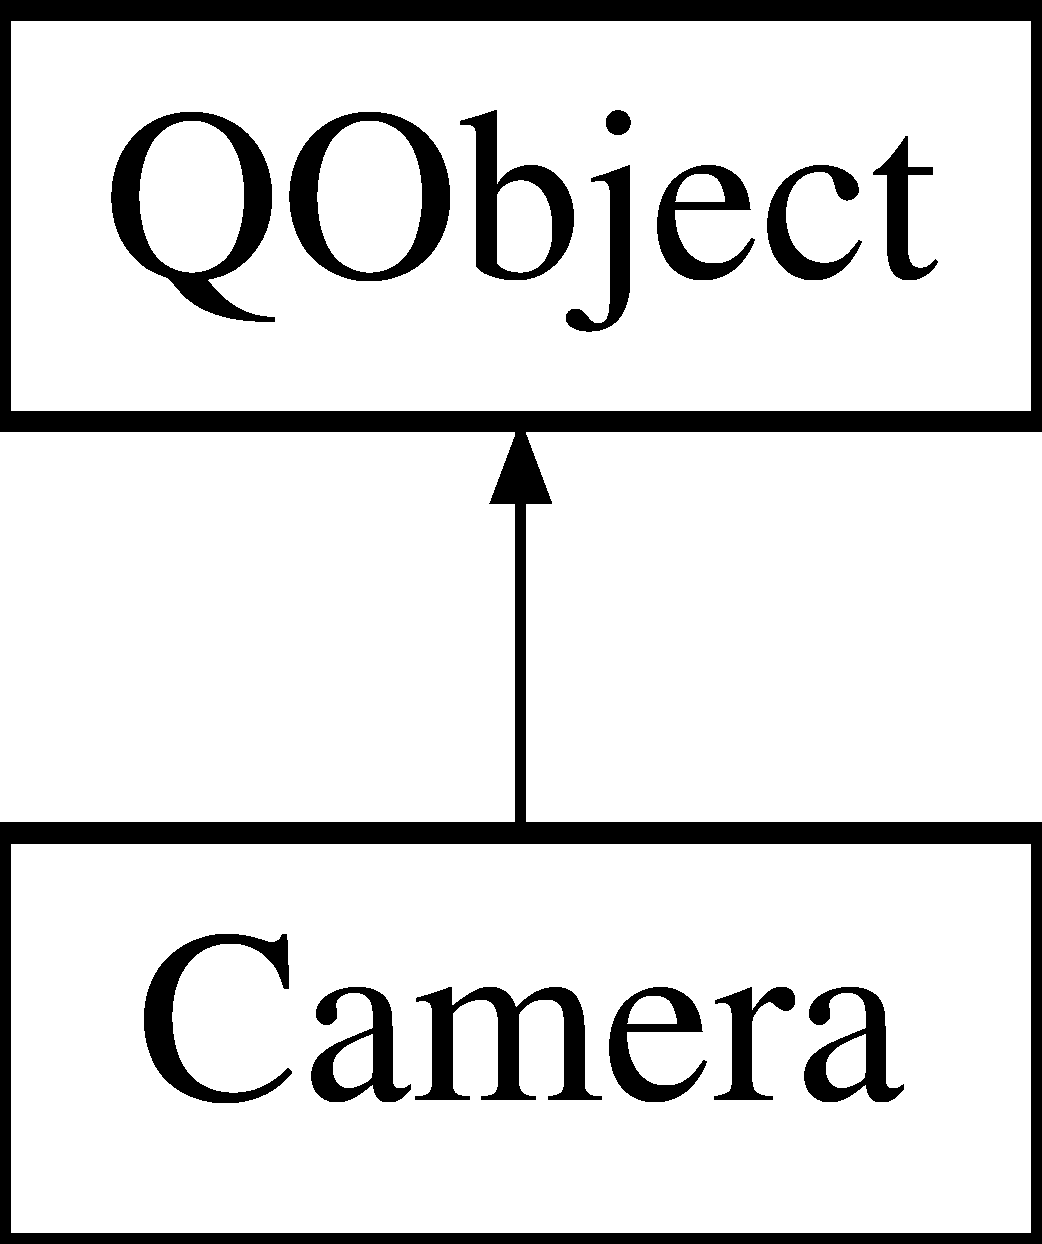
\includegraphics[height=2.000000cm]{class_camera}
\end{center}
\end{figure}
\subsection*{Public Slots}
\begin{DoxyCompactItemize}
\item 
void \hyperlink{class_camera_ab54c500b9e9cb8281bf89e15b767b3ac}{update\+Ratio} (int width, int height)
\begin{DoxyCompactList}\small\item\em update\+Ratio updates the aspect\+Ratio for the Projection of the \hyperlink{class_camera}{Camera}. This shoud be updated when the screen size changes. \end{DoxyCompactList}\end{DoxyCompactItemize}
\subsection*{Public Member Functions}
\begin{DoxyCompactItemize}
\item 
\hyperlink{class_camera_a3ac5bf011721a2b688e5ce077e4ee2e8}{Camera} (int width=1, int height=1)
\begin{DoxyCompactList}\small\item\em \hyperlink{class_camera}{Camera} Creates a new \hyperlink{class_camera}{Camera} with standard values. \end{DoxyCompactList}\item 
Q\+Matrix4x4 \hyperlink{class_camera_a1dd0e418636627fca41d061ef82d869d}{get\+World\+To\+View\+Matrix} () const 
\begin{DoxyCompactList}\small\item\em get\+World\+To\+View\+Matrix generates the World to View Matrix for this \hyperlink{class_camera}{Camera} \end{DoxyCompactList}\item 
Q\+Matrix4x4 \hyperlink{class_camera_aebc04996f3f393bdf98a8034d8f10a03}{get\+View\+To\+Projection\+Matrix} () const 
\begin{DoxyCompactList}\small\item\em get\+View\+To\+Projection\+Matrix generates the Projection Matrix for this \hyperlink{class_camera}{Camera} \end{DoxyCompactList}\end{DoxyCompactItemize}


\subsection{Detailed Description}
The \hyperlink{class_camera}{Camera} class Class for a \hyperlink{class_camera}{Camera} in a 3\+D \hyperlink{class_scene}{Scene} The \hyperlink{class_camera}{Camera} Calculates the World to View Matrix and the Projection Matrix. 

\hyperlink{class_camera}{Camera} is initilzed with standard values

T\+O\+D\+O\+: Need function to change values 

Definition at line 15 of file camera.\+h.



\subsection{Constructor \& Destructor Documentation}
\hypertarget{class_camera_a3ac5bf011721a2b688e5ce077e4ee2e8}{}\index{Camera@{Camera}!Camera@{Camera}}
\index{Camera@{Camera}!Camera@{Camera}}
\subsubsection[{Camera(int width=1, int height=1)}]{\setlength{\rightskip}{0pt plus 5cm}Camera\+::\+Camera (
\begin{DoxyParamCaption}
\item[{int}]{width = {\ttfamily 1}, }
\item[{int}]{height = {\ttfamily 1}}
\end{DoxyParamCaption}
)}\label{class_camera_a3ac5bf011721a2b688e5ce077e4ee2e8}


\hyperlink{class_camera}{Camera} Creates a new \hyperlink{class_camera}{Camera} with standard values. 


\begin{DoxyParams}{Parameters}
{\em width} & width of the screen for the correct aspect\+Ratio \\
\hline
{\em height} & height of the screen for the correct aspect\+Ratio \\
\hline
\end{DoxyParams}


Definition at line 3 of file camera.\+cpp.



\subsection{Member Function Documentation}
\hypertarget{class_camera_aebc04996f3f393bdf98a8034d8f10a03}{}\index{Camera@{Camera}!get\+View\+To\+Projection\+Matrix@{get\+View\+To\+Projection\+Matrix}}
\index{get\+View\+To\+Projection\+Matrix@{get\+View\+To\+Projection\+Matrix}!Camera@{Camera}}
\subsubsection[{get\+View\+To\+Projection\+Matrix() const }]{\setlength{\rightskip}{0pt plus 5cm}Q\+Matrix4x4 Camera\+::get\+View\+To\+Projection\+Matrix (
\begin{DoxyParamCaption}
{}
\end{DoxyParamCaption}
) const}\label{class_camera_aebc04996f3f393bdf98a8034d8f10a03}


get\+View\+To\+Projection\+Matrix generates the Projection Matrix for this \hyperlink{class_camera}{Camera} 

\begin{DoxyReturn}{Returns}
Q\+Matrix4x4\} 
\end{DoxyReturn}


Definition at line 20 of file camera.\+cpp.

\hypertarget{class_camera_a1dd0e418636627fca41d061ef82d869d}{}\index{Camera@{Camera}!get\+World\+To\+View\+Matrix@{get\+World\+To\+View\+Matrix}}
\index{get\+World\+To\+View\+Matrix@{get\+World\+To\+View\+Matrix}!Camera@{Camera}}
\subsubsection[{get\+World\+To\+View\+Matrix() const }]{\setlength{\rightskip}{0pt plus 5cm}Q\+Matrix4x4 Camera\+::get\+World\+To\+View\+Matrix (
\begin{DoxyParamCaption}
{}
\end{DoxyParamCaption}
) const}\label{class_camera_a1dd0e418636627fca41d061ef82d869d}


get\+World\+To\+View\+Matrix generates the World to View Matrix for this \hyperlink{class_camera}{Camera} 

\begin{DoxyReturn}{Returns}
Q\+Matrix4x4\} World\+To\+View\+Matrix 
\end{DoxyReturn}


Definition at line 13 of file camera.\+cpp.

\hypertarget{class_camera_ab54c500b9e9cb8281bf89e15b767b3ac}{}\index{Camera@{Camera}!update\+Ratio@{update\+Ratio}}
\index{update\+Ratio@{update\+Ratio}!Camera@{Camera}}
\subsubsection[{update\+Ratio}]{\setlength{\rightskip}{0pt plus 5cm}void Camera\+::update\+Ratio (
\begin{DoxyParamCaption}
\item[{int}]{width, }
\item[{int}]{height}
\end{DoxyParamCaption}
)\hspace{0.3cm}{\ttfamily [inline]}, {\ttfamily [slot]}}\label{class_camera_ab54c500b9e9cb8281bf89e15b767b3ac}


update\+Ratio updates the aspect\+Ratio for the Projection of the \hyperlink{class_camera}{Camera}. This shoud be updated when the screen size changes. 


\begin{DoxyParams}{Parameters}
{\em width} & int new width of the screen device \\
\hline
{\em height} & int new height of the screen devce \\
\hline
\end{DoxyParams}


Definition at line 55 of file camera.\+h.



The documentation for this class was generated from the following files\+:\begin{DoxyCompactItemize}
\item 
\hyperlink{camera_8h}{camera.\+h}\item 
\hyperlink{camera_8cpp}{camera.\+cpp}\end{DoxyCompactItemize}

\hypertarget{class_entity}{}\section{Entity Class Reference}
\label{class_entity}\index{Entity@{Entity}}


The \hyperlink{class_entity}{Entity} class.  




{\ttfamily \#include $<$entity.\+h$>$}

Inheritance diagram for Entity\+:\begin{figure}[H]
\begin{center}
\leavevmode
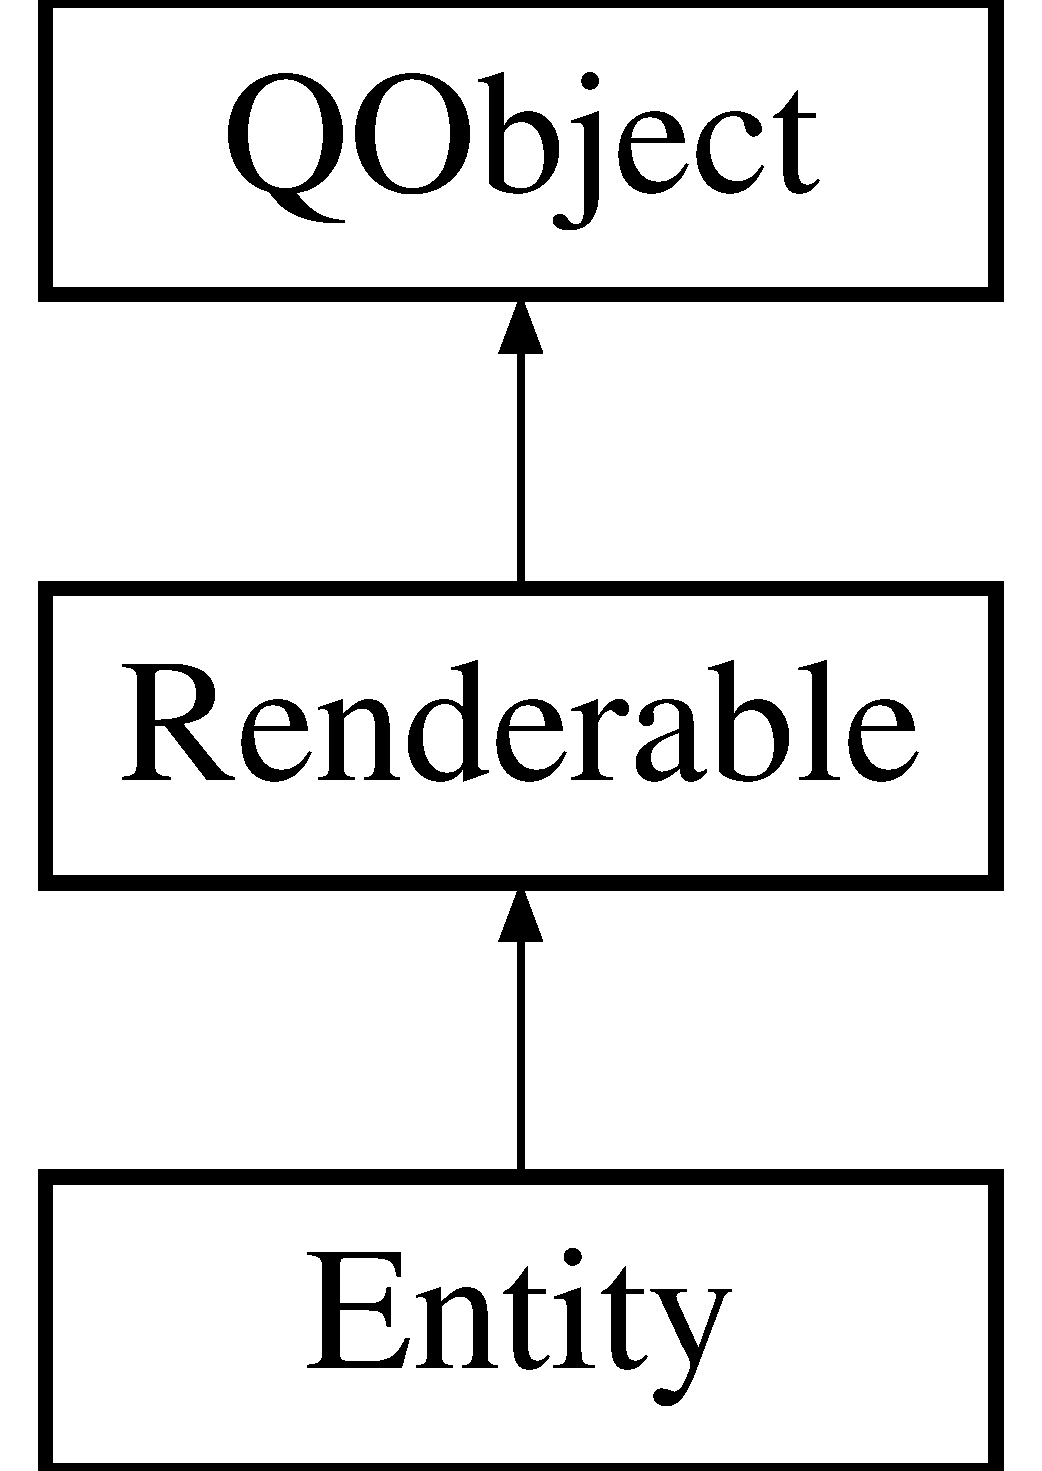
\includegraphics[height=3.000000cm]{class_entity}
\end{center}
\end{figure}
\subsection*{Public Member Functions}
\begin{DoxyCompactItemize}
\item 
\hyperlink{class_entity_acf4f8570960b2173a894a99ec9967215}{Entity} (\hyperlink{class_mesh}{Mesh} $\ast$p\+Mesh, \hyperlink{class_material}{Material} $\ast$p\+Material, Q\+Open\+G\+L\+Context $\ast$context, const Q\+Matrix4x4 $\ast$p\+World, const Q\+String str\+Name=\char`\"{}Entity\char`\"{}, Q\+Object $\ast$parent=0)
\begin{DoxyCompactList}\small\item\em \hyperlink{class_entity}{Entity} creates a new \hyperlink{class_entity}{Entity} need a \hyperlink{class_mesh}{Mesh}, \hyperlink{class_material}{Material}, Context and a Position in the World. \end{DoxyCompactList}\item 
\hyperlink{class_entity_adf6d3f7cb1b2ba029b6b048a395cc8ae}{$\sim$\+Entity} ()
\item 
virtual void \hyperlink{class_entity_a647d154620c6464168f3b088f0ac170e}{Create} ()
\begin{DoxyCompactList}\small\item\em Create and initilize Open\+G\+L Values Creates \hyperlink{class_mesh}{Mesh} and \hyperlink{class_material}{Material} and initilize them. \end{DoxyCompactList}\item 
virtual void \hyperlink{class_entity_aa75151fc607686b42d27f8c3ba73143d}{Destroy} ()
\begin{DoxyCompactList}\small\item\em Destroy Clear the G\+P\+U Memory and Delets the Open\+G\+L Values. \end{DoxyCompactList}\item 
virtual void \hyperlink{class_entity_a0f3f11bbb868ab96e5bbb0f835eb9966}{Render} (G\+Luint draw\+Order, const Q\+Matrix4x4 $\ast$p\+View, const Q\+Matrix4x4 $\ast$p\+Proj, const \hyperlink{class_light}{Light} $\ast$light)
\begin{DoxyCompactList}\small\item\em Render Renders the \hyperlink{class_entity}{Entity} to the given open\+G\+L context. \end{DoxyCompactList}\end{DoxyCompactItemize}
\subsection*{Protected Attributes}
\begin{DoxyCompactItemize}
\item 
\hyperlink{class_material}{Material} $\ast$ \hyperlink{class_entity_adbbe41659ac87bbed15c53e6101292e8}{material}
\item 
\hyperlink{class_mesh}{Mesh} $\ast$ \hyperlink{class_entity_ab346a9ce19733368f64f9109fb290ff1}{mesh}
\item 
Q\+Open\+G\+L\+Vertex\+Array\+Object $\ast$ \hyperlink{class_entity_aaddc09c82caf2a17d745af5283771eac}{gl\+V\+A\+O}
\item 
Q\+Matrix4x4 \hyperlink{class_entity_ad9ec1327cacd74787dd951ff4389ca15}{world\+To\+View}
\item 
Q\+Matrix4x4 \hyperlink{class_entity_adddbfb9b19b765cb9674ad95fe9f22ce}{view\+To\+Projecton}
\end{DoxyCompactItemize}


\subsection{Detailed Description}
The \hyperlink{class_entity}{Entity} class. 

Implements a \hyperlink{class_renderable}{Renderable} Object a \hyperlink{class_renderable}{Renderable} \hyperlink{class_mesh}{Mesh} with one \hyperlink{class_material}{Material}

\begin{DoxySeeAlso}{See also}
\hyperlink{class_mesh}{Mesh} 

\hyperlink{class_material}{Material} 
\end{DoxySeeAlso}


Definition at line 19 of file entity.\+h.



\subsection{Constructor \& Destructor Documentation}
\hypertarget{class_entity_acf4f8570960b2173a894a99ec9967215}{}\index{Entity@{Entity}!Entity@{Entity}}
\index{Entity@{Entity}!Entity@{Entity}}
\subsubsection[{Entity(\+Mesh $\ast$p\+Mesh, Material $\ast$p\+Material, Q\+Open\+G\+L\+Context $\ast$context, const Q\+Matrix4x4 $\ast$p\+World, const Q\+String str\+Name=""Entity"", Q\+Object $\ast$parent=0)}]{\setlength{\rightskip}{0pt plus 5cm}Entity\+::\+Entity (
\begin{DoxyParamCaption}
\item[{{\bf Mesh} $\ast$}]{p\+Mesh, }
\item[{{\bf Material} $\ast$}]{p\+Material, }
\item[{Q\+Open\+G\+L\+Context $\ast$}]{context, }
\item[{const Q\+Matrix4x4 $\ast$}]{p\+World, }
\item[{const Q\+String}]{str\+Name = {\ttfamily \char`\"{}Entity\char`\"{}}, }
\item[{Q\+Object $\ast$}]{parent = {\ttfamily 0}}
\end{DoxyParamCaption}
)}\label{class_entity_acf4f8570960b2173a894a99ec9967215}


\hyperlink{class_entity}{Entity} creates a new \hyperlink{class_entity}{Entity} need a \hyperlink{class_mesh}{Mesh}, \hyperlink{class_material}{Material}, Context and a Position in the World. 


\begin{DoxyParams}{Parameters}
{\em p\+Mesh} & the \hyperlink{class_mesh}{Mesh} of the \hyperlink{class_entity}{Entity} \\
\hline
{\em p\+Material} & the \hyperlink{class_material}{Material} for the \hyperlink{class_mesh}{Mesh} \\
\hline
{\em context} & the context witch shoud be drawed to \\
\hline
{\em p\+World} & the model\+To\+World Matrix gives the position of the Entiry in the World \\
\hline
{\em str\+Name} & O\+P\+T. gives the \hyperlink{class_entity}{Entity} a name \\
\hline
{\em parent} & O\+P\+T Q\+Object Parent \\
\hline
\end{DoxyParams}


Definition at line 8 of file entity.\+cpp.

\hypertarget{class_entity_adf6d3f7cb1b2ba029b6b048a395cc8ae}{}\index{Entity@{Entity}!````~Entity@{$\sim$\+Entity}}
\index{````~Entity@{$\sim$\+Entity}!Entity@{Entity}}
\subsubsection[{$\sim$\+Entity()}]{\setlength{\rightskip}{0pt plus 5cm}Entity\+::$\sim$\+Entity (
\begin{DoxyParamCaption}
{}
\end{DoxyParamCaption}
)}\label{class_entity_adf6d3f7cb1b2ba029b6b048a395cc8ae}


Definition at line 70 of file entity.\+cpp.



\subsection{Member Function Documentation}
\hypertarget{class_entity_a647d154620c6464168f3b088f0ac170e}{}\index{Entity@{Entity}!Create@{Create}}
\index{Create@{Create}!Entity@{Entity}}
\subsubsection[{Create()}]{\setlength{\rightskip}{0pt plus 5cm}void Entity\+::\+Create (
\begin{DoxyParamCaption}
{}
\end{DoxyParamCaption}
)\hspace{0.3cm}{\ttfamily [virtual]}}\label{class_entity_a647d154620c6464168f3b088f0ac170e}


Create and initilize Open\+G\+L Values Creates \hyperlink{class_mesh}{Mesh} and \hyperlink{class_material}{Material} and initilize them. 



Implements \hyperlink{class_renderable_ab204246b39a34b14a3f258a065cc3019}{Renderable}.



Definition at line 20 of file entity.\+cpp.

\hypertarget{class_entity_aa75151fc607686b42d27f8c3ba73143d}{}\index{Entity@{Entity}!Destroy@{Destroy}}
\index{Destroy@{Destroy}!Entity@{Entity}}
\subsubsection[{Destroy()}]{\setlength{\rightskip}{0pt plus 5cm}void Entity\+::\+Destroy (
\begin{DoxyParamCaption}
{}
\end{DoxyParamCaption}
)\hspace{0.3cm}{\ttfamily [virtual]}}\label{class_entity_aa75151fc607686b42d27f8c3ba73143d}


Destroy Clear the G\+P\+U Memory and Delets the Open\+G\+L Values. 



Implements \hyperlink{class_renderable_aaf8e0b324e35f8a1b61a9667a0d91d51}{Renderable}.



Definition at line 64 of file entity.\+cpp.

\hypertarget{class_entity_a0f3f11bbb868ab96e5bbb0f835eb9966}{}\index{Entity@{Entity}!Render@{Render}}
\index{Render@{Render}!Entity@{Entity}}
\subsubsection[{Render(\+G\+Luint draw\+Order, const Q\+Matrix4x4 $\ast$p\+View, const Q\+Matrix4x4 $\ast$p\+Proj, const Light $\ast$light)}]{\setlength{\rightskip}{0pt plus 5cm}void Entity\+::\+Render (
\begin{DoxyParamCaption}
\item[{G\+Luint}]{draw\+Order, }
\item[{const Q\+Matrix4x4 $\ast$}]{p\+View, }
\item[{const Q\+Matrix4x4 $\ast$}]{p\+Proj, }
\item[{const {\bf Light} $\ast$}]{light}
\end{DoxyParamCaption}
)\hspace{0.3cm}{\ttfamily [virtual]}}\label{class_entity_a0f3f11bbb868ab96e5bbb0f835eb9966}


Render Renders the \hyperlink{class_entity}{Entity} to the given open\+G\+L context. 


\begin{DoxyParams}{Parameters}
{\em draw\+Order} & order \\
\hline
{\em p\+View} & World\+To\+View Matrix for the \hyperlink{class_entity}{Entity} \\
\hline
{\em p\+Proj} & Projection for the \hyperlink{class_entity}{Entity} \\
\hline
{\em light} & A light for rendering \\
\hline
\end{DoxyParams}


Implements \hyperlink{class_renderable_aee9a55d459edefe6c8b8532ab5d7102c}{Renderable}.



Definition at line 36 of file entity.\+cpp.



\subsection{Member Data Documentation}
\hypertarget{class_entity_aaddc09c82caf2a17d745af5283771eac}{}\index{Entity@{Entity}!gl\+V\+A\+O@{gl\+V\+A\+O}}
\index{gl\+V\+A\+O@{gl\+V\+A\+O}!Entity@{Entity}}
\subsubsection[{gl\+V\+A\+O}]{\setlength{\rightskip}{0pt plus 5cm}Q\+Open\+G\+L\+Vertex\+Array\+Object$\ast$ Entity\+::gl\+V\+A\+O\hspace{0.3cm}{\ttfamily [protected]}}\label{class_entity_aaddc09c82caf2a17d745af5283771eac}


Definition at line 25 of file entity.\+h.

\hypertarget{class_entity_adbbe41659ac87bbed15c53e6101292e8}{}\index{Entity@{Entity}!material@{material}}
\index{material@{material}!Entity@{Entity}}
\subsubsection[{material}]{\setlength{\rightskip}{0pt plus 5cm}{\bf Material}$\ast$ Entity\+::material\hspace{0.3cm}{\ttfamily [protected]}}\label{class_entity_adbbe41659ac87bbed15c53e6101292e8}


Definition at line 23 of file entity.\+h.

\hypertarget{class_entity_ab346a9ce19733368f64f9109fb290ff1}{}\index{Entity@{Entity}!mesh@{mesh}}
\index{mesh@{mesh}!Entity@{Entity}}
\subsubsection[{mesh}]{\setlength{\rightskip}{0pt plus 5cm}{\bf Mesh}$\ast$ Entity\+::mesh\hspace{0.3cm}{\ttfamily [protected]}}\label{class_entity_ab346a9ce19733368f64f9109fb290ff1}


Definition at line 24 of file entity.\+h.

\hypertarget{class_entity_adddbfb9b19b765cb9674ad95fe9f22ce}{}\index{Entity@{Entity}!view\+To\+Projecton@{view\+To\+Projecton}}
\index{view\+To\+Projecton@{view\+To\+Projecton}!Entity@{Entity}}
\subsubsection[{view\+To\+Projecton}]{\setlength{\rightskip}{0pt plus 5cm}Q\+Matrix4x4 Entity\+::view\+To\+Projecton\hspace{0.3cm}{\ttfamily [protected]}}\label{class_entity_adddbfb9b19b765cb9674ad95fe9f22ce}


Definition at line 29 of file entity.\+h.

\hypertarget{class_entity_ad9ec1327cacd74787dd951ff4389ca15}{}\index{Entity@{Entity}!world\+To\+View@{world\+To\+View}}
\index{world\+To\+View@{world\+To\+View}!Entity@{Entity}}
\subsubsection[{world\+To\+View}]{\setlength{\rightskip}{0pt plus 5cm}Q\+Matrix4x4 Entity\+::world\+To\+View\hspace{0.3cm}{\ttfamily [protected]}}\label{class_entity_ad9ec1327cacd74787dd951ff4389ca15}


Definition at line 28 of file entity.\+h.



The documentation for this class was generated from the following files\+:\begin{DoxyCompactItemize}
\item 
\hyperlink{entity_8h}{entity.\+h}\item 
\hyperlink{entity_8cpp}{entity.\+cpp}\end{DoxyCompactItemize}

\hypertarget{class_light}{}\section{Light Class Reference}
\label{class_light}\index{Light@{Light}}


The \hyperlink{class_light}{Light} class holding Values for diffrent light Types The Shader choose with type is used.  




{\ttfamily \#include $<$light.\+h$>$}

\subsection*{Public Member Functions}
\begin{DoxyCompactItemize}
\item 
Q\+Vector3\+D \hyperlink{class_light_abc98e7a0deaef970249b24b99fbfe2af}{get\+Ambient\+Color} () const 
\item 
void \hyperlink{class_light_ab1d1e7a1f677eac15b3fee85af6e19af}{set\+Ambient\+Color} (const Q\+Vector3\+D \&value)
\item 
Q\+Vector3\+D \hyperlink{class_light_a1fd761051fe5ae7e0b63ccb9a2e70559}{get\+Diffuse\+Color} () const 
\item 
void \hyperlink{class_light_ad9622cbcca5b9918094b29ae1e3e11d0}{set\+Diffuse\+Color} (const Q\+Vector3\+D \&value)
\item 
Q\+Vector3\+D \hyperlink{class_light_a58a17d6d8c1e107425a548f151e95eb6}{get\+Direction} () const 
\item 
void \hyperlink{class_light_a59366d8b8970a990a1a7ec10089c66f9}{set\+Direction} (const Q\+Vector3\+D \&value)
\item 
Q\+Vector3\+D \hyperlink{class_light_a0755863d1018d6dae555765d1698854e}{get\+Position} () const 
\item 
Q\+Vector4\+D \hyperlink{class_light_ad73fb358c98f26624bdf6476267ff56b}{get\+Attenstion} () const 
\item 
void \hyperlink{class_light_a4955734440953fd7ea593cf6f7734113}{set\+Attenstion} (const Q\+Vector4\+D \&value)
\item 
float \hyperlink{class_light_a26c205e4785b96e13017c8bec807b406}{get\+Cos\+Half\+Phi} () const 
\item 
void \hyperlink{class_light_ae801b5a8477448649e741051a97c4476}{set\+Cos\+Half\+Phi} (float value)
\item 
float \hyperlink{class_light_af8d37302912489269b84d8b1981f8295}{get\+Cos\+Half\+Theta} () const 
\item 
void \hyperlink{class_light_a6da8d4a84ee9492412525c317c9e37fd}{set\+Cos\+Half\+Theta} (float value)
\item 
\hyperlink{class_light_aeb5df09a25a32f19fdffa761268ba24f}{Light} ()
\begin{DoxyCompactList}\small\item\em \hyperlink{class_light}{Light} Creates a new \hyperlink{class_light}{Light} with normal values. \end{DoxyCompactList}\end{DoxyCompactItemize}
\subsection*{Protected Attributes}
\begin{DoxyCompactItemize}
\item 
Q\+Vector3\+D \hyperlink{class_light_ab4989464d97bfcfecea32f2a89181be7}{position}
\item 
Q\+Vector3\+D \hyperlink{class_light_ae3a1c33d67bfb4fa2e16ce5e5b2021a4}{direction}
\item 
Q\+Vector3\+D \hyperlink{class_light_a4e0f72de18d88038e3d9e8c0b5318ec7}{diffuse\+Color}
\item 
Q\+Vector3\+D \hyperlink{class_light_a4613929744a5de8828ed660fca90366f}{ambient\+Color}
\item 
Q\+Vector4\+D \hyperlink{class_light_aee062fbeac40aa71642450f016aac961}{attenstion}
\item 
float \hyperlink{class_light_ab91ec48042aa2f542231a7225b0e55fe}{cos\+Half\+Phi}
\item 
float \hyperlink{class_light_a4c5aa51610a4c60375ddc247fe71c422}{cos\+Half\+Theta}
\end{DoxyCompactItemize}


\subsection{Detailed Description}
The \hyperlink{class_light}{Light} class holding Values for diffrent light Types The Shader choose with type is used. 

Definition at line 12 of file light.\+h.



\subsection{Constructor \& Destructor Documentation}
\hypertarget{class_light_aeb5df09a25a32f19fdffa761268ba24f}{}\index{Light@{Light}!Light@{Light}}
\index{Light@{Light}!Light@{Light}}
\subsubsection[{Light()}]{\setlength{\rightskip}{0pt plus 5cm}Light\+::\+Light (
\begin{DoxyParamCaption}
{}
\end{DoxyParamCaption}
)}\label{class_light_aeb5df09a25a32f19fdffa761268ba24f}


\hyperlink{class_light}{Light} Creates a new \hyperlink{class_light}{Light} with normal values. 



Definition at line 3 of file light.\+cpp.



\subsection{Member Function Documentation}
\hypertarget{class_light_abc98e7a0deaef970249b24b99fbfe2af}{}\index{Light@{Light}!get\+Ambient\+Color@{get\+Ambient\+Color}}
\index{get\+Ambient\+Color@{get\+Ambient\+Color}!Light@{Light}}
\subsubsection[{get\+Ambient\+Color() const }]{\setlength{\rightskip}{0pt plus 5cm}Q\+Vector3\+D Light\+::get\+Ambient\+Color (
\begin{DoxyParamCaption}
{}
\end{DoxyParamCaption}
) const}\label{class_light_abc98e7a0deaef970249b24b99fbfe2af}


Definition at line 10 of file light.\+cpp.

\hypertarget{class_light_ad73fb358c98f26624bdf6476267ff56b}{}\index{Light@{Light}!get\+Attenstion@{get\+Attenstion}}
\index{get\+Attenstion@{get\+Attenstion}!Light@{Light}}
\subsubsection[{get\+Attenstion() const }]{\setlength{\rightskip}{0pt plus 5cm}Q\+Vector4\+D Light\+::get\+Attenstion (
\begin{DoxyParamCaption}
{}
\end{DoxyParamCaption}
) const}\label{class_light_ad73fb358c98f26624bdf6476267ff56b}


Definition at line 45 of file light.\+cpp.

\hypertarget{class_light_a26c205e4785b96e13017c8bec807b406}{}\index{Light@{Light}!get\+Cos\+Half\+Phi@{get\+Cos\+Half\+Phi}}
\index{get\+Cos\+Half\+Phi@{get\+Cos\+Half\+Phi}!Light@{Light}}
\subsubsection[{get\+Cos\+Half\+Phi() const }]{\setlength{\rightskip}{0pt plus 5cm}float Light\+::get\+Cos\+Half\+Phi (
\begin{DoxyParamCaption}
{}
\end{DoxyParamCaption}
) const}\label{class_light_a26c205e4785b96e13017c8bec807b406}


Definition at line 55 of file light.\+cpp.

\hypertarget{class_light_af8d37302912489269b84d8b1981f8295}{}\index{Light@{Light}!get\+Cos\+Half\+Theta@{get\+Cos\+Half\+Theta}}
\index{get\+Cos\+Half\+Theta@{get\+Cos\+Half\+Theta}!Light@{Light}}
\subsubsection[{get\+Cos\+Half\+Theta() const }]{\setlength{\rightskip}{0pt plus 5cm}float Light\+::get\+Cos\+Half\+Theta (
\begin{DoxyParamCaption}
{}
\end{DoxyParamCaption}
) const}\label{class_light_af8d37302912489269b84d8b1981f8295}


Definition at line 65 of file light.\+cpp.

\hypertarget{class_light_a1fd761051fe5ae7e0b63ccb9a2e70559}{}\index{Light@{Light}!get\+Diffuse\+Color@{get\+Diffuse\+Color}}
\index{get\+Diffuse\+Color@{get\+Diffuse\+Color}!Light@{Light}}
\subsubsection[{get\+Diffuse\+Color() const }]{\setlength{\rightskip}{0pt plus 5cm}Q\+Vector3\+D Light\+::get\+Diffuse\+Color (
\begin{DoxyParamCaption}
{}
\end{DoxyParamCaption}
) const}\label{class_light_a1fd761051fe5ae7e0b63ccb9a2e70559}


Definition at line 20 of file light.\+cpp.

\hypertarget{class_light_a58a17d6d8c1e107425a548f151e95eb6}{}\index{Light@{Light}!get\+Direction@{get\+Direction}}
\index{get\+Direction@{get\+Direction}!Light@{Light}}
\subsubsection[{get\+Direction() const }]{\setlength{\rightskip}{0pt plus 5cm}Q\+Vector3\+D Light\+::get\+Direction (
\begin{DoxyParamCaption}
{}
\end{DoxyParamCaption}
) const}\label{class_light_a58a17d6d8c1e107425a548f151e95eb6}


Definition at line 30 of file light.\+cpp.

\hypertarget{class_light_a0755863d1018d6dae555765d1698854e}{}\index{Light@{Light}!get\+Position@{get\+Position}}
\index{get\+Position@{get\+Position}!Light@{Light}}
\subsubsection[{get\+Position() const }]{\setlength{\rightskip}{0pt plus 5cm}Q\+Vector3\+D Light\+::get\+Position (
\begin{DoxyParamCaption}
{}
\end{DoxyParamCaption}
) const}\label{class_light_a0755863d1018d6dae555765d1698854e}


Definition at line 40 of file light.\+cpp.

\hypertarget{class_light_ab1d1e7a1f677eac15b3fee85af6e19af}{}\index{Light@{Light}!set\+Ambient\+Color@{set\+Ambient\+Color}}
\index{set\+Ambient\+Color@{set\+Ambient\+Color}!Light@{Light}}
\subsubsection[{set\+Ambient\+Color(const Q\+Vector3\+D \&value)}]{\setlength{\rightskip}{0pt plus 5cm}void Light\+::set\+Ambient\+Color (
\begin{DoxyParamCaption}
\item[{const Q\+Vector3\+D \&}]{value}
\end{DoxyParamCaption}
)}\label{class_light_ab1d1e7a1f677eac15b3fee85af6e19af}


Definition at line 15 of file light.\+cpp.

\hypertarget{class_light_a4955734440953fd7ea593cf6f7734113}{}\index{Light@{Light}!set\+Attenstion@{set\+Attenstion}}
\index{set\+Attenstion@{set\+Attenstion}!Light@{Light}}
\subsubsection[{set\+Attenstion(const Q\+Vector4\+D \&value)}]{\setlength{\rightskip}{0pt plus 5cm}void Light\+::set\+Attenstion (
\begin{DoxyParamCaption}
\item[{const Q\+Vector4\+D \&}]{value}
\end{DoxyParamCaption}
)}\label{class_light_a4955734440953fd7ea593cf6f7734113}


Definition at line 50 of file light.\+cpp.

\hypertarget{class_light_ae801b5a8477448649e741051a97c4476}{}\index{Light@{Light}!set\+Cos\+Half\+Phi@{set\+Cos\+Half\+Phi}}
\index{set\+Cos\+Half\+Phi@{set\+Cos\+Half\+Phi}!Light@{Light}}
\subsubsection[{set\+Cos\+Half\+Phi(float value)}]{\setlength{\rightskip}{0pt plus 5cm}void Light\+::set\+Cos\+Half\+Phi (
\begin{DoxyParamCaption}
\item[{float}]{value}
\end{DoxyParamCaption}
)}\label{class_light_ae801b5a8477448649e741051a97c4476}


Definition at line 60 of file light.\+cpp.

\hypertarget{class_light_a6da8d4a84ee9492412525c317c9e37fd}{}\index{Light@{Light}!set\+Cos\+Half\+Theta@{set\+Cos\+Half\+Theta}}
\index{set\+Cos\+Half\+Theta@{set\+Cos\+Half\+Theta}!Light@{Light}}
\subsubsection[{set\+Cos\+Half\+Theta(float value)}]{\setlength{\rightskip}{0pt plus 5cm}void Light\+::set\+Cos\+Half\+Theta (
\begin{DoxyParamCaption}
\item[{float}]{value}
\end{DoxyParamCaption}
)}\label{class_light_a6da8d4a84ee9492412525c317c9e37fd}


Definition at line 70 of file light.\+cpp.

\hypertarget{class_light_ad9622cbcca5b9918094b29ae1e3e11d0}{}\index{Light@{Light}!set\+Diffuse\+Color@{set\+Diffuse\+Color}}
\index{set\+Diffuse\+Color@{set\+Diffuse\+Color}!Light@{Light}}
\subsubsection[{set\+Diffuse\+Color(const Q\+Vector3\+D \&value)}]{\setlength{\rightskip}{0pt plus 5cm}void Light\+::set\+Diffuse\+Color (
\begin{DoxyParamCaption}
\item[{const Q\+Vector3\+D \&}]{value}
\end{DoxyParamCaption}
)}\label{class_light_ad9622cbcca5b9918094b29ae1e3e11d0}


Definition at line 25 of file light.\+cpp.

\hypertarget{class_light_a59366d8b8970a990a1a7ec10089c66f9}{}\index{Light@{Light}!set\+Direction@{set\+Direction}}
\index{set\+Direction@{set\+Direction}!Light@{Light}}
\subsubsection[{set\+Direction(const Q\+Vector3\+D \&value)}]{\setlength{\rightskip}{0pt plus 5cm}void Light\+::set\+Direction (
\begin{DoxyParamCaption}
\item[{const Q\+Vector3\+D \&}]{value}
\end{DoxyParamCaption}
)}\label{class_light_a59366d8b8970a990a1a7ec10089c66f9}


Definition at line 35 of file light.\+cpp.



\subsection{Member Data Documentation}
\hypertarget{class_light_a4613929744a5de8828ed660fca90366f}{}\index{Light@{Light}!ambient\+Color@{ambient\+Color}}
\index{ambient\+Color@{ambient\+Color}!Light@{Light}}
\subsubsection[{ambient\+Color}]{\setlength{\rightskip}{0pt plus 5cm}Q\+Vector3\+D Light\+::ambient\+Color\hspace{0.3cm}{\ttfamily [protected]}}\label{class_light_a4613929744a5de8828ed660fca90366f}


Definition at line 18 of file light.\+h.

\hypertarget{class_light_aee062fbeac40aa71642450f016aac961}{}\index{Light@{Light}!attenstion@{attenstion}}
\index{attenstion@{attenstion}!Light@{Light}}
\subsubsection[{attenstion}]{\setlength{\rightskip}{0pt plus 5cm}Q\+Vector4\+D Light\+::attenstion\hspace{0.3cm}{\ttfamily [protected]}}\label{class_light_aee062fbeac40aa71642450f016aac961}


Definition at line 21 of file light.\+h.

\hypertarget{class_light_ab91ec48042aa2f542231a7225b0e55fe}{}\index{Light@{Light}!cos\+Half\+Phi@{cos\+Half\+Phi}}
\index{cos\+Half\+Phi@{cos\+Half\+Phi}!Light@{Light}}
\subsubsection[{cos\+Half\+Phi}]{\setlength{\rightskip}{0pt plus 5cm}float Light\+::cos\+Half\+Phi\hspace{0.3cm}{\ttfamily [protected]}}\label{class_light_ab91ec48042aa2f542231a7225b0e55fe}


Definition at line 24 of file light.\+h.

\hypertarget{class_light_a4c5aa51610a4c60375ddc247fe71c422}{}\index{Light@{Light}!cos\+Half\+Theta@{cos\+Half\+Theta}}
\index{cos\+Half\+Theta@{cos\+Half\+Theta}!Light@{Light}}
\subsubsection[{cos\+Half\+Theta}]{\setlength{\rightskip}{0pt plus 5cm}float Light\+::cos\+Half\+Theta\hspace{0.3cm}{\ttfamily [protected]}}\label{class_light_a4c5aa51610a4c60375ddc247fe71c422}


Definition at line 25 of file light.\+h.

\hypertarget{class_light_a4e0f72de18d88038e3d9e8c0b5318ec7}{}\index{Light@{Light}!diffuse\+Color@{diffuse\+Color}}
\index{diffuse\+Color@{diffuse\+Color}!Light@{Light}}
\subsubsection[{diffuse\+Color}]{\setlength{\rightskip}{0pt plus 5cm}Q\+Vector3\+D Light\+::diffuse\+Color\hspace{0.3cm}{\ttfamily [protected]}}\label{class_light_a4e0f72de18d88038e3d9e8c0b5318ec7}


Definition at line 17 of file light.\+h.

\hypertarget{class_light_ae3a1c33d67bfb4fa2e16ce5e5b2021a4}{}\index{Light@{Light}!direction@{direction}}
\index{direction@{direction}!Light@{Light}}
\subsubsection[{direction}]{\setlength{\rightskip}{0pt plus 5cm}Q\+Vector3\+D Light\+::direction\hspace{0.3cm}{\ttfamily [protected]}}\label{class_light_ae3a1c33d67bfb4fa2e16ce5e5b2021a4}


Definition at line 16 of file light.\+h.

\hypertarget{class_light_ab4989464d97bfcfecea32f2a89181be7}{}\index{Light@{Light}!position@{position}}
\index{position@{position}!Light@{Light}}
\subsubsection[{position}]{\setlength{\rightskip}{0pt plus 5cm}Q\+Vector3\+D Light\+::position\hspace{0.3cm}{\ttfamily [protected]}}\label{class_light_ab4989464d97bfcfecea32f2a89181be7}


Definition at line 15 of file light.\+h.



The documentation for this class was generated from the following files\+:\begin{DoxyCompactItemize}
\item 
\hyperlink{light_8h}{light.\+h}\item 
\hyperlink{light_8cpp}{light.\+cpp}\end{DoxyCompactItemize}

\hypertarget{class_material}{}\section{Material Class Reference}
\label{class_material}\index{Material@{Material}}


The \hyperlink{class_material}{Material} class.  




{\ttfamily \#include $<$material.\+h$>$}

Inheritance diagram for Material\+:\begin{figure}[H]
\begin{center}
\leavevmode
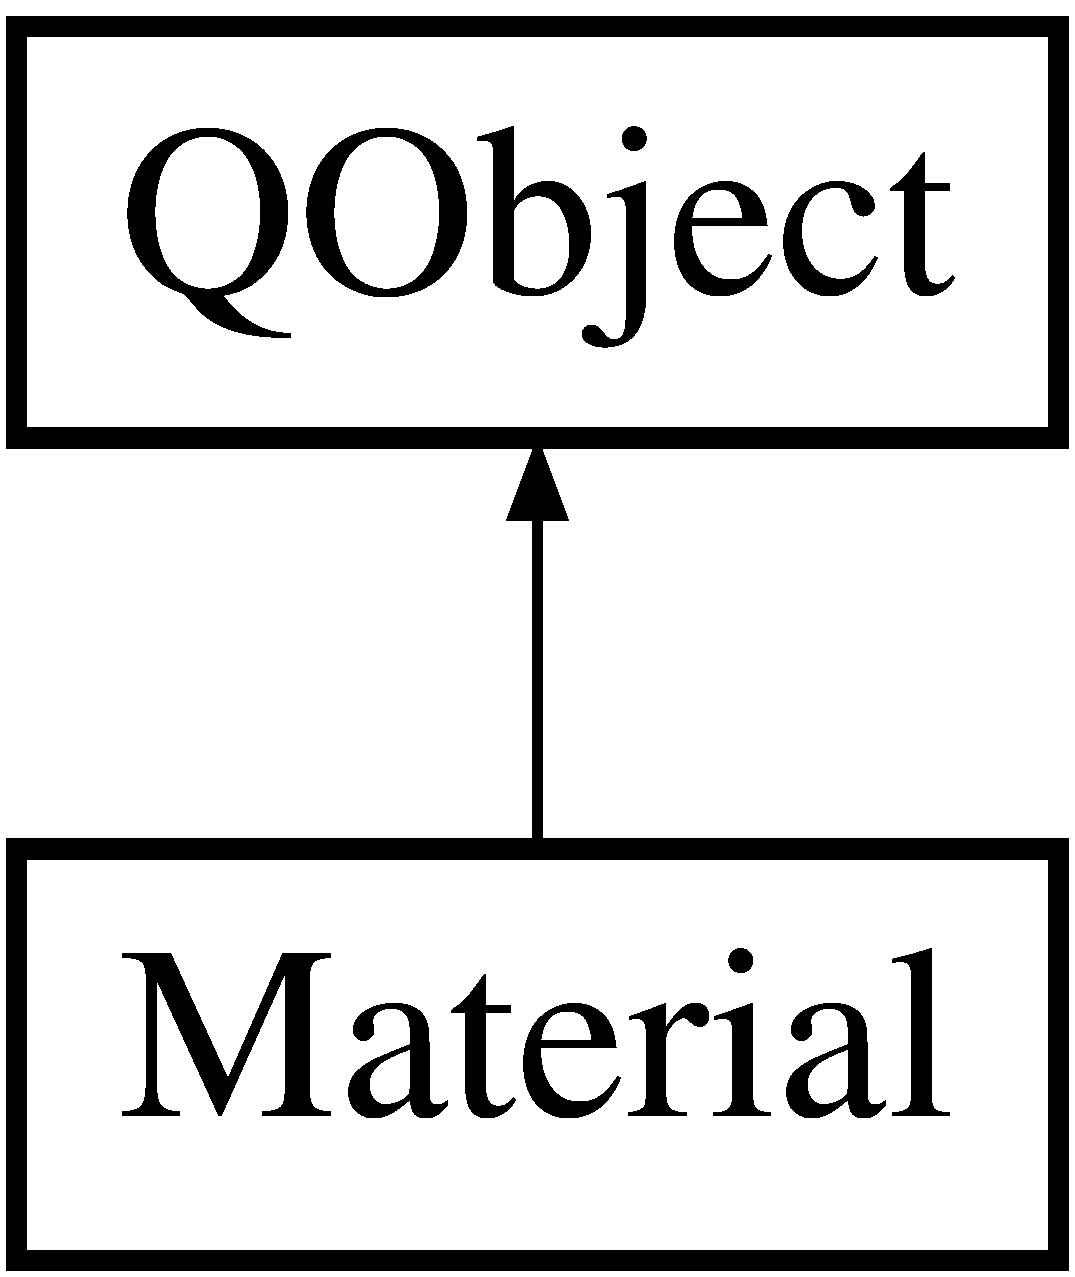
\includegraphics[height=2.000000cm]{class_material}
\end{center}
\end{figure}
\subsection*{Public Member Functions}
\begin{DoxyCompactItemize}
\item 
\hyperlink{class_material_a70259ad64e743ee286bddd3bb0389a28}{Material} (Q\+Open\+G\+L\+Context $\ast$context, Q\+String v\+Shader\+File, Q\+String f\+Shader\+File, Q\+Object $\ast$parent=0)
\begin{DoxyCompactList}\small\item\em \hyperlink{class_material_a70259ad64e743ee286bddd3bb0389a28}{Material\+::\+Material} Creates a new \hyperlink{class_material}{Material} there are no shaders compiled or liked or bound. \end{DoxyCompactList}\item 
virtual void \hyperlink{class_material_af39de221a1c5a6ebe920d732e3c84b40}{Create} ()
\begin{DoxyCompactList}\small\item\em \hyperlink{class_material_af39de221a1c5a6ebe920d732e3c84b40}{Material\+::\+Create} reads the shader files, compiles them and adds them to a programm. \end{DoxyCompactList}\item 
virtual void \hyperlink{class_material_aeee87ae4ec3829e9e32119f557c59753}{Destroy} ()
\begin{DoxyCompactList}\small\item\em \hyperlink{class_material_aeee87ae4ec3829e9e32119f557c59753}{Material\+::\+Destroy} deletes the shaders and programm. \end{DoxyCompactList}\item 
virtual void \hyperlink{class_material_a8eff0925974e755d3a9a216a8063c3de}{Create\+Vertex\+Layout} (\hyperlink{class_mesh}{Mesh} $\ast$format)
\begin{DoxyCompactList}\small\item\em \hyperlink{class_material_a8eff0925974e755d3a9a216a8063c3de}{Material\+::\+Create\+Vertex\+Layout} binds \hyperlink{class_material}{Material} to a Vertex\+Buffer and sets up the data structure. \end{DoxyCompactList}\item 
virtual void \hyperlink{class_material_a031a68217b55fb3c46a01757c58eb836}{Setup} ()
\begin{DoxyCompactList}\small\item\em \hyperlink{class_material_a031a68217b55fb3c46a01757c58eb836}{Material\+::\+Setup} Setup shader values for the hole material livetime. \end{DoxyCompactList}\item 
virtual void \hyperlink{class_material_a3b2ab993eed57211d14f16f71efe6b75}{Setup\+Per\+Object} (const Q\+Matrix4x4 $\ast$mat\+World, const Q\+Matrix4x4 $\ast$mat\+World\+View, const Q\+Matrix4x4 $\ast$mat\+World\+View\+Projection)
\begin{DoxyCompactList}\small\item\em \hyperlink{class_material_a3b2ab993eed57211d14f16f71efe6b75}{Material\+::\+Setup\+Per\+Object} Setup values that needed to be setup for one object for one time. \end{DoxyCompactList}\item 
virtual void \hyperlink{class_material_a56025231f7fe57d5cf68fd21d2d425a1}{Setup\+Per\+Frame} (const \hyperlink{class_light}{Light} $\ast$p\+Light)
\begin{DoxyCompactList}\small\item\em \hyperlink{class_material_a56025231f7fe57d5cf68fd21d2d425a1}{Material\+::\+Setup\+Per\+Frame} Setup \hyperlink{class_material}{Material} Values (e.\+g. the \hyperlink{class_light}{Light} source) that need to be updates only one a Frame not for every Object. \end{DoxyCompactList}\item 
Q\+Open\+G\+L\+Shader $\ast$ \hyperlink{class_material_ad67cd89b791d35c26bdd8b9e4f486790}{get\+Vertex\+Shader} ()
\item 
Q\+Open\+G\+L\+Shader $\ast$ \hyperlink{class_material_a21f6b7cacf4e6fd64e3976951a296fb7}{get\+Fragment\+Shader} ()
\item 
Q\+Open\+G\+L\+Shader\+Program $\ast$ \hyperlink{class_material_a9ee8bb9a9370af4b0ab7790f5802c38a}{get\+Shader\+Programm} ()
\item 
void \hyperlink{class_material_a0abb21c533c69ea57fabc48d593db9af}{set\+Diffuse\+Color} (const Q\+Vector4\+D \&value)
\item 
void \hyperlink{class_material_a0c1cf0dcdd31f2a5ee6ccdef7a049216}{set\+Ambient\+Color} (const Q\+Vector4\+D \&value)
\end{DoxyCompactItemize}
\subsection*{Protected Attributes}
\begin{DoxyCompactItemize}
\item 
Q\+Open\+G\+L\+Context $\ast$ \hyperlink{class_material_a83da87bdd6d755b6f8ed40929001d355}{context\+Device}
\item 
Q\+String \hyperlink{class_material_af8361fc71a1f55c5a49100bee94bd94a}{vertex\+Shader\+File\+Name}
\item 
Q\+String \hyperlink{class_material_a8adf8679e41e341b339f3460c3ba45ee}{fragment\+Shader\+File\+Name}
\item 
Q\+Open\+G\+L\+Shader $\ast$ \hyperlink{class_material_af7fc01b5cbebefdc983797f60cd4772c}{vertex\+Shader}
\item 
Q\+Open\+G\+L\+Shader $\ast$ \hyperlink{class_material_a9a2cb05e65584fa9d4f0f4f0af74d55e}{fragment\+Shader}
\item 
Q\+Open\+G\+L\+Shader\+Program $\ast$ \hyperlink{class_material_aa5f04d76a6b53bfb6eba238db8328490}{programm}
\item 
Q\+Vector4\+D \hyperlink{class_material_a38b1cde46c908ae719ebaf9de1efb5ff}{diffuse\+Color}
\item 
Q\+Vector4\+D \hyperlink{class_material_aabbefbcb0d05f0ae4521eb68183ff702}{ambient\+Color}
\item 
int \hyperlink{class_material_ad4963cc03e54c2e539a98b60070d2beb}{diffuse\+Color\+Location}
\item 
int \hyperlink{class_material_a938adfa6b527c7462df99493968f14aa}{ambient\+Color\+Location}
\item 
int \hyperlink{class_material_ac1241a29b62d04848cdc190f1de85849}{vertex\+Location}
\item 
int \hyperlink{class_material_a12a1db7e857ec3bcbacbcd646f5cd16f}{world\+View\+Proj\+Matrix\+Location}
\end{DoxyCompactItemize}


\subsection{Detailed Description}
The \hyperlink{class_material}{Material} class. 

This Class manages a material for a Object. A \hyperlink{class_material}{Material} contains vertex and fragment shader and manages the connection to them 

Definition at line 19 of file material.\+h.



\subsection{Constructor \& Destructor Documentation}
\hypertarget{class_material_a70259ad64e743ee286bddd3bb0389a28}{}\index{Material@{Material}!Material@{Material}}
\index{Material@{Material}!Material@{Material}}
\subsubsection[{Material(\+Q\+Open\+G\+L\+Context $\ast$context, Q\+String v\+Shader\+File, Q\+String f\+Shader\+File, Q\+Object $\ast$parent=0)}]{\setlength{\rightskip}{0pt plus 5cm}Material\+::\+Material (
\begin{DoxyParamCaption}
\item[{Q\+Open\+G\+L\+Context $\ast$}]{context, }
\item[{Q\+String}]{v\+Shader\+File, }
\item[{Q\+String}]{f\+Shader\+File, }
\item[{Q\+Object $\ast$}]{parent = {\ttfamily 0}}
\end{DoxyParamCaption}
)\hspace{0.3cm}{\ttfamily [explicit]}}\label{class_material_a70259ad64e743ee286bddd3bb0389a28}


\hyperlink{class_material_a70259ad64e743ee286bddd3bb0389a28}{Material\+::\+Material} Creates a new \hyperlink{class_material}{Material} there are no shaders compiled or liked or bound. 


\begin{DoxyParams}{Parameters}
{\em context} & open\+Gl context for the \hyperlink{class_material}{Material} \\
\hline
{\em v\+Shader\+File} & Vertex-\/\+Shader file name and location \\
\hline
{\em f\+Shader\+File} & Fragment-\/\+Shader file name and location \\
\hline
{\em parent} & \\
\hline
\end{DoxyParams}


Definition at line 13 of file material.\+cpp.



\subsection{Member Function Documentation}
\hypertarget{class_material_af39de221a1c5a6ebe920d732e3c84b40}{}\index{Material@{Material}!Create@{Create}}
\index{Create@{Create}!Material@{Material}}
\subsubsection[{Create()}]{\setlength{\rightskip}{0pt plus 5cm}void Material\+::\+Create (
\begin{DoxyParamCaption}
{}
\end{DoxyParamCaption}
)\hspace{0.3cm}{\ttfamily [virtual]}}\label{class_material_af39de221a1c5a6ebe920d732e3c84b40}


\hyperlink{class_material_af39de221a1c5a6ebe920d732e3c84b40}{Material\+::\+Create} reads the shader files, compiles them and adds them to a programm. 



Definition at line 34 of file material.\+cpp.

\hypertarget{class_material_a8eff0925974e755d3a9a216a8063c3de}{}\index{Material@{Material}!Create\+Vertex\+Layout@{Create\+Vertex\+Layout}}
\index{Create\+Vertex\+Layout@{Create\+Vertex\+Layout}!Material@{Material}}
\subsubsection[{Create\+Vertex\+Layout(\+Mesh $\ast$format)}]{\setlength{\rightskip}{0pt plus 5cm}void Material\+::\+Create\+Vertex\+Layout (
\begin{DoxyParamCaption}
\item[{{\bf Mesh} $\ast$}]{format}
\end{DoxyParamCaption}
)\hspace{0.3cm}{\ttfamily [virtual]}}\label{class_material_a8eff0925974e755d3a9a216a8063c3de}


\hyperlink{class_material_a8eff0925974e755d3a9a216a8063c3de}{Material\+::\+Create\+Vertex\+Layout} binds \hyperlink{class_material}{Material} to a Vertex\+Buffer and sets up the data structure. 


\begin{DoxyParams}{Parameters}
{\em vertex\+Buffer} & Q\+Open\+G\+L\+Buffer with the Vertex\+Buffer \\
\hline
{\em format} & Vertex\+Format says what format the Buffer has with color etc \\
\hline
\end{DoxyParams}


Definition at line 77 of file material.\+cpp.

\hypertarget{class_material_aeee87ae4ec3829e9e32119f557c59753}{}\index{Material@{Material}!Destroy@{Destroy}}
\index{Destroy@{Destroy}!Material@{Material}}
\subsubsection[{Destroy()}]{\setlength{\rightskip}{0pt plus 5cm}void Material\+::\+Destroy (
\begin{DoxyParamCaption}
{}
\end{DoxyParamCaption}
)\hspace{0.3cm}{\ttfamily [virtual]}}\label{class_material_aeee87ae4ec3829e9e32119f557c59753}


\hyperlink{class_material_aeee87ae4ec3829e9e32119f557c59753}{Material\+::\+Destroy} deletes the shaders and programm. 



Definition at line 61 of file material.\+cpp.

\hypertarget{class_material_a21f6b7cacf4e6fd64e3976951a296fb7}{}\index{Material@{Material}!get\+Fragment\+Shader@{get\+Fragment\+Shader}}
\index{get\+Fragment\+Shader@{get\+Fragment\+Shader}!Material@{Material}}
\subsubsection[{get\+Fragment\+Shader()}]{\setlength{\rightskip}{0pt plus 5cm}Q\+Open\+G\+L\+Shader$\ast$ Material\+::get\+Fragment\+Shader (
\begin{DoxyParamCaption}
{}
\end{DoxyParamCaption}
)\hspace{0.3cm}{\ttfamily [inline]}}\label{class_material_a21f6b7cacf4e6fd64e3976951a296fb7}


Definition at line 58 of file material.\+h.

\hypertarget{class_material_a9ee8bb9a9370af4b0ab7790f5802c38a}{}\index{Material@{Material}!get\+Shader\+Programm@{get\+Shader\+Programm}}
\index{get\+Shader\+Programm@{get\+Shader\+Programm}!Material@{Material}}
\subsubsection[{get\+Shader\+Programm()}]{\setlength{\rightskip}{0pt plus 5cm}Q\+Open\+G\+L\+Shader\+Program$\ast$ Material\+::get\+Shader\+Programm (
\begin{DoxyParamCaption}
{}
\end{DoxyParamCaption}
)\hspace{0.3cm}{\ttfamily [inline]}}\label{class_material_a9ee8bb9a9370af4b0ab7790f5802c38a}


Definition at line 59 of file material.\+h.

\hypertarget{class_material_ad67cd89b791d35c26bdd8b9e4f486790}{}\index{Material@{Material}!get\+Vertex\+Shader@{get\+Vertex\+Shader}}
\index{get\+Vertex\+Shader@{get\+Vertex\+Shader}!Material@{Material}}
\subsubsection[{get\+Vertex\+Shader()}]{\setlength{\rightskip}{0pt plus 5cm}Q\+Open\+G\+L\+Shader$\ast$ Material\+::get\+Vertex\+Shader (
\begin{DoxyParamCaption}
{}
\end{DoxyParamCaption}
)\hspace{0.3cm}{\ttfamily [inline]}}\label{class_material_ad67cd89b791d35c26bdd8b9e4f486790}


Definition at line 57 of file material.\+h.

\hypertarget{class_material_a0c1cf0dcdd31f2a5ee6ccdef7a049216}{}\index{Material@{Material}!set\+Ambient\+Color@{set\+Ambient\+Color}}
\index{set\+Ambient\+Color@{set\+Ambient\+Color}!Material@{Material}}
\subsubsection[{set\+Ambient\+Color(const Q\+Vector4\+D \&value)}]{\setlength{\rightskip}{0pt plus 5cm}void Material\+::set\+Ambient\+Color (
\begin{DoxyParamCaption}
\item[{const Q\+Vector4\+D \&}]{value}
\end{DoxyParamCaption}
)\hspace{0.3cm}{\ttfamily [inline]}}\label{class_material_a0c1cf0dcdd31f2a5ee6ccdef7a049216}


Definition at line 65 of file material.\+h.

\hypertarget{class_material_a0abb21c533c69ea57fabc48d593db9af}{}\index{Material@{Material}!set\+Diffuse\+Color@{set\+Diffuse\+Color}}
\index{set\+Diffuse\+Color@{set\+Diffuse\+Color}!Material@{Material}}
\subsubsection[{set\+Diffuse\+Color(const Q\+Vector4\+D \&value)}]{\setlength{\rightskip}{0pt plus 5cm}void Material\+::set\+Diffuse\+Color (
\begin{DoxyParamCaption}
\item[{const Q\+Vector4\+D \&}]{value}
\end{DoxyParamCaption}
)\hspace{0.3cm}{\ttfamily [inline]}}\label{class_material_a0abb21c533c69ea57fabc48d593db9af}


Definition at line 62 of file material.\+h.

\hypertarget{class_material_a031a68217b55fb3c46a01757c58eb836}{}\index{Material@{Material}!Setup@{Setup}}
\index{Setup@{Setup}!Material@{Material}}
\subsubsection[{Setup()}]{\setlength{\rightskip}{0pt plus 5cm}void Material\+::\+Setup (
\begin{DoxyParamCaption}
{}
\end{DoxyParamCaption}
)\hspace{0.3cm}{\ttfamily [virtual]}}\label{class_material_a031a68217b55fb3c46a01757c58eb836}


\hyperlink{class_material_a031a68217b55fb3c46a01757c58eb836}{Material\+::\+Setup} Setup shader values for the hole material livetime. 



Definition at line 96 of file material.\+cpp.

\hypertarget{class_material_a56025231f7fe57d5cf68fd21d2d425a1}{}\index{Material@{Material}!Setup\+Per\+Frame@{Setup\+Per\+Frame}}
\index{Setup\+Per\+Frame@{Setup\+Per\+Frame}!Material@{Material}}
\subsubsection[{Setup\+Per\+Frame(const Light $\ast$p\+Light)}]{\setlength{\rightskip}{0pt plus 5cm}void Material\+::\+Setup\+Per\+Frame (
\begin{DoxyParamCaption}
\item[{const {\bf Light} $\ast$}]{p\+Light}
\end{DoxyParamCaption}
)\hspace{0.3cm}{\ttfamily [virtual]}}\label{class_material_a56025231f7fe57d5cf68fd21d2d425a1}


\hyperlink{class_material_a56025231f7fe57d5cf68fd21d2d425a1}{Material\+::\+Setup\+Per\+Frame} Setup \hyperlink{class_material}{Material} Values (e.\+g. the \hyperlink{class_light}{Light} source) that need to be updates only one a Frame not for every Object. 


\begin{DoxyParams}{Parameters}
{\em p\+Light} & light values; \\
\hline
\end{DoxyParams}


Definition at line 128 of file material.\+cpp.

\hypertarget{class_material_a3b2ab993eed57211d14f16f71efe6b75}{}\index{Material@{Material}!Setup\+Per\+Object@{Setup\+Per\+Object}}
\index{Setup\+Per\+Object@{Setup\+Per\+Object}!Material@{Material}}
\subsubsection[{Setup\+Per\+Object(const Q\+Matrix4x4 $\ast$mat\+World, const Q\+Matrix4x4 $\ast$mat\+World\+View, const Q\+Matrix4x4 $\ast$mat\+World\+View\+Projection)}]{\setlength{\rightskip}{0pt plus 5cm}void Material\+::\+Setup\+Per\+Object (
\begin{DoxyParamCaption}
\item[{const Q\+Matrix4x4 $\ast$}]{mat\+World, }
\item[{const Q\+Matrix4x4 $\ast$}]{mat\+World\+View, }
\item[{const Q\+Matrix4x4 $\ast$}]{mat\+World\+View\+Projection}
\end{DoxyParamCaption}
)\hspace{0.3cm}{\ttfamily [virtual]}}\label{class_material_a3b2ab993eed57211d14f16f71efe6b75}


\hyperlink{class_material_a3b2ab993eed57211d14f16f71efe6b75}{Material\+::\+Setup\+Per\+Object} Setup values that needed to be setup for one object for one time. 


\begin{DoxyParams}{Parameters}
{\em mat\+World} & Q\+Matrix4x4\}$\ast$ The World matrix for that object \\
\hline
{\em mat\+World\+View} & Q\+Matrix4x4\}$\ast$ The World\+View matrix for that object \\
\hline
{\em mat\+World\+View\+Projection} & Q\+Matrix4x4\}$\ast$ The World\+View\+Projection matrix for that object \\
\hline
\end{DoxyParams}


Definition at line 114 of file material.\+cpp.



\subsection{Member Data Documentation}
\hypertarget{class_material_aabbefbcb0d05f0ae4521eb68183ff702}{}\index{Material@{Material}!ambient\+Color@{ambient\+Color}}
\index{ambient\+Color@{ambient\+Color}!Material@{Material}}
\subsubsection[{ambient\+Color}]{\setlength{\rightskip}{0pt plus 5cm}Q\+Vector4\+D Material\+::ambient\+Color\hspace{0.3cm}{\ttfamily [protected]}}\label{class_material_aabbefbcb0d05f0ae4521eb68183ff702}


Definition at line 36 of file material.\+h.

\hypertarget{class_material_a938adfa6b527c7462df99493968f14aa}{}\index{Material@{Material}!ambient\+Color\+Location@{ambient\+Color\+Location}}
\index{ambient\+Color\+Location@{ambient\+Color\+Location}!Material@{Material}}
\subsubsection[{ambient\+Color\+Location}]{\setlength{\rightskip}{0pt plus 5cm}int Material\+::ambient\+Color\+Location\hspace{0.3cm}{\ttfamily [protected]}}\label{class_material_a938adfa6b527c7462df99493968f14aa}


Definition at line 39 of file material.\+h.

\hypertarget{class_material_a83da87bdd6d755b6f8ed40929001d355}{}\index{Material@{Material}!context\+Device@{context\+Device}}
\index{context\+Device@{context\+Device}!Material@{Material}}
\subsubsection[{context\+Device}]{\setlength{\rightskip}{0pt plus 5cm}Q\+Open\+G\+L\+Context$\ast$ Material\+::context\+Device\hspace{0.3cm}{\ttfamily [protected]}}\label{class_material_a83da87bdd6d755b6f8ed40929001d355}


Definition at line 25 of file material.\+h.

\hypertarget{class_material_a38b1cde46c908ae719ebaf9de1efb5ff}{}\index{Material@{Material}!diffuse\+Color@{diffuse\+Color}}
\index{diffuse\+Color@{diffuse\+Color}!Material@{Material}}
\subsubsection[{diffuse\+Color}]{\setlength{\rightskip}{0pt plus 5cm}Q\+Vector4\+D Material\+::diffuse\+Color\hspace{0.3cm}{\ttfamily [protected]}}\label{class_material_a38b1cde46c908ae719ebaf9de1efb5ff}


Definition at line 35 of file material.\+h.

\hypertarget{class_material_ad4963cc03e54c2e539a98b60070d2beb}{}\index{Material@{Material}!diffuse\+Color\+Location@{diffuse\+Color\+Location}}
\index{diffuse\+Color\+Location@{diffuse\+Color\+Location}!Material@{Material}}
\subsubsection[{diffuse\+Color\+Location}]{\setlength{\rightskip}{0pt plus 5cm}int Material\+::diffuse\+Color\+Location\hspace{0.3cm}{\ttfamily [protected]}}\label{class_material_ad4963cc03e54c2e539a98b60070d2beb}


Definition at line 38 of file material.\+h.

\hypertarget{class_material_a9a2cb05e65584fa9d4f0f4f0af74d55e}{}\index{Material@{Material}!fragment\+Shader@{fragment\+Shader}}
\index{fragment\+Shader@{fragment\+Shader}!Material@{Material}}
\subsubsection[{fragment\+Shader}]{\setlength{\rightskip}{0pt plus 5cm}Q\+Open\+G\+L\+Shader$\ast$ Material\+::fragment\+Shader\hspace{0.3cm}{\ttfamily [protected]}}\label{class_material_a9a2cb05e65584fa9d4f0f4f0af74d55e}


Definition at line 31 of file material.\+h.

\hypertarget{class_material_a8adf8679e41e341b339f3460c3ba45ee}{}\index{Material@{Material}!fragment\+Shader\+File\+Name@{fragment\+Shader\+File\+Name}}
\index{fragment\+Shader\+File\+Name@{fragment\+Shader\+File\+Name}!Material@{Material}}
\subsubsection[{fragment\+Shader\+File\+Name}]{\setlength{\rightskip}{0pt plus 5cm}Q\+String Material\+::fragment\+Shader\+File\+Name\hspace{0.3cm}{\ttfamily [protected]}}\label{class_material_a8adf8679e41e341b339f3460c3ba45ee}


Definition at line 28 of file material.\+h.

\hypertarget{class_material_aa5f04d76a6b53bfb6eba238db8328490}{}\index{Material@{Material}!programm@{programm}}
\index{programm@{programm}!Material@{Material}}
\subsubsection[{programm}]{\setlength{\rightskip}{0pt plus 5cm}Q\+Open\+G\+L\+Shader\+Program$\ast$ Material\+::programm\hspace{0.3cm}{\ttfamily [protected]}}\label{class_material_aa5f04d76a6b53bfb6eba238db8328490}


Definition at line 33 of file material.\+h.

\hypertarget{class_material_ac1241a29b62d04848cdc190f1de85849}{}\index{Material@{Material}!vertex\+Location@{vertex\+Location}}
\index{vertex\+Location@{vertex\+Location}!Material@{Material}}
\subsubsection[{vertex\+Location}]{\setlength{\rightskip}{0pt plus 5cm}int Material\+::vertex\+Location\hspace{0.3cm}{\ttfamily [protected]}}\label{class_material_ac1241a29b62d04848cdc190f1de85849}


Definition at line 40 of file material.\+h.

\hypertarget{class_material_af7fc01b5cbebefdc983797f60cd4772c}{}\index{Material@{Material}!vertex\+Shader@{vertex\+Shader}}
\index{vertex\+Shader@{vertex\+Shader}!Material@{Material}}
\subsubsection[{vertex\+Shader}]{\setlength{\rightskip}{0pt plus 5cm}Q\+Open\+G\+L\+Shader$\ast$ Material\+::vertex\+Shader\hspace{0.3cm}{\ttfamily [protected]}}\label{class_material_af7fc01b5cbebefdc983797f60cd4772c}


Definition at line 30 of file material.\+h.

\hypertarget{class_material_af8361fc71a1f55c5a49100bee94bd94a}{}\index{Material@{Material}!vertex\+Shader\+File\+Name@{vertex\+Shader\+File\+Name}}
\index{vertex\+Shader\+File\+Name@{vertex\+Shader\+File\+Name}!Material@{Material}}
\subsubsection[{vertex\+Shader\+File\+Name}]{\setlength{\rightskip}{0pt plus 5cm}Q\+String Material\+::vertex\+Shader\+File\+Name\hspace{0.3cm}{\ttfamily [protected]}}\label{class_material_af8361fc71a1f55c5a49100bee94bd94a}


Definition at line 27 of file material.\+h.

\hypertarget{class_material_a12a1db7e857ec3bcbacbcd646f5cd16f}{}\index{Material@{Material}!world\+View\+Proj\+Matrix\+Location@{world\+View\+Proj\+Matrix\+Location}}
\index{world\+View\+Proj\+Matrix\+Location@{world\+View\+Proj\+Matrix\+Location}!Material@{Material}}
\subsubsection[{world\+View\+Proj\+Matrix\+Location}]{\setlength{\rightskip}{0pt plus 5cm}int Material\+::world\+View\+Proj\+Matrix\+Location\hspace{0.3cm}{\ttfamily [protected]}}\label{class_material_a12a1db7e857ec3bcbacbcd646f5cd16f}


Definition at line 41 of file material.\+h.



The documentation for this class was generated from the following files\+:\begin{DoxyCompactItemize}
\item 
\hyperlink{material_8h}{material.\+h}\item 
\hyperlink{material_8cpp}{material.\+cpp}\end{DoxyCompactItemize}

\hypertarget{class_mesh}{}\section{Mesh Class Reference}
\label{class_mesh}\index{Mesh@{Mesh}}


The \hyperlink{class_mesh}{Mesh} class Contains all vertex Information abstract Interface.  




{\ttfamily \#include $<$mesh.\+h$>$}

Inheritance diagram for Mesh\+:\begin{figure}[H]
\begin{center}
\leavevmode
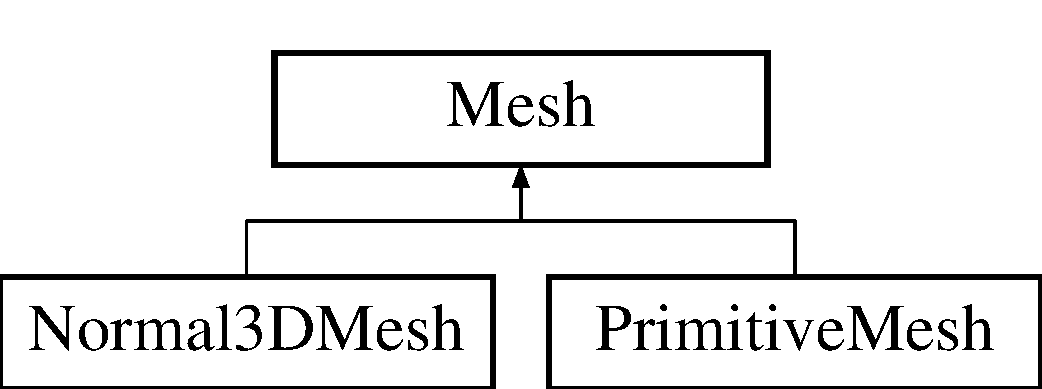
\includegraphics[height=2.000000cm]{class_mesh}
\end{center}
\end{figure}
\subsection*{Public Member Functions}
\begin{DoxyCompactItemize}
\item 
virtual int \hyperlink{class_mesh_a525d8b7c9ff840a0a92c507f0ff2febf}{vertex\+Size} ()
\item 
virtual int \hyperlink{class_mesh_a93afbbcbeaa686dc6a4ae342e842f530}{index\+Size} ()
\item 
virtual float $\ast$ \hyperlink{class_mesh_a7086a32bd045e773e636da12e4f9c1b4}{vertex} ()
\item 
virtual int \hyperlink{class_mesh_a112080d5664bb21790632b7bfcafb4f4}{vertex\+Tupel} ()
\item 
virtual int \hyperlink{class_mesh_abf79b0e9fff121f85f6b2163e8c053f9}{vertex\+Stride} ()
\item 
virtual int \hyperlink{class_mesh_a999026dae1d89c13f5e27a886271d028}{vertex\+Offset} ()
\item 
virtual G\+Lushort $\ast$ \hyperlink{class_mesh_a85b1d83752f168ff75d8327e5dd89df4}{indecies} ()
\item 
virtual int \hyperlink{class_mesh_a1ad488fd8f2d6395f645a127273f0a90}{index\+Stride} ()
\item 
virtual int \hyperlink{class_mesh_abdf32aa39510ff70e9a1d23daebe0c43}{index\+Offset} ()
\item 
virtual void \hyperlink{class_mesh_a8fe3f7dd50c087fe472c0b75ba423974}{bind} ()
\item 
virtual void \hyperlink{class_mesh_a747251d7e9e44fcd7bfd58a89bba7e61}{release} ()
\item 
virtual void \hyperlink{class_mesh_a4e113d785d96bb8b36695469f4c5d862}{Create} ()
\begin{DoxyCompactList}\small\item\em Create the Open\+G\+L buffer objects for This \hyperlink{class_mesh}{Mesh} from the mesh data and sends this data to the G\+P\+U. \end{DoxyCompactList}\item 
virtual void \hyperlink{class_mesh_a969df8ef15def20cfc48c265d194b3c2}{Destroy} ()
\begin{DoxyCompactList}\small\item\em Destroy Removes the Open\+G\+L buffers for this \hyperlink{class_mesh}{Mesh} from the G\+P\+U. \end{DoxyCompactList}\end{DoxyCompactItemize}
\subsection*{Protected Member Functions}
\begin{DoxyCompactItemize}
\item 
\hyperlink{class_mesh_a2af137f1571af89172b9c102302c416b}{Mesh} ()
\end{DoxyCompactItemize}
\subsection*{Protected Attributes}
\begin{DoxyCompactItemize}
\item 
Q\+Open\+G\+L\+Buffer $\ast$ \hyperlink{class_mesh_ae53507ed0f2756e37a55e57a169cbec0}{vertex\+Buffer}
\item 
Q\+Open\+G\+L\+Buffer $\ast$ \hyperlink{class_mesh_a4b4a752380875f7ade2301f656a45a51}{index\+Buffer}
\item 
int \hyperlink{class_mesh_a840028792aecdad5f9b649222329d521}{v\+Size}
\item 
int \hyperlink{class_mesh_ac6283b99dbb698e2efd83357278b06b7}{i\+Size}
\item 
int \hyperlink{class_mesh_a07d24d28a6cf55b5575e0525dd9ecceb}{v\+Tupel}
\item 
int \hyperlink{class_mesh_a5e054aa2a4f8e2af8f1f5342ef847f26}{v\+Stride}
\item 
int \hyperlink{class_mesh_a251ab9a090efb842f2b5e2674d31e112}{v\+Offset}
\item 
int \hyperlink{class_mesh_afe2f0742c0ef6088eaf38b87a8896392}{i\+Stride}
\item 
int \hyperlink{class_mesh_a8837e5a3b75f17b5ebab3b67928489ce}{i\+Offset}
\item 
Q\+Vector3\+D $\ast$ \hyperlink{class_mesh_a32d007d7d539832b7feb35e11ff4586c}{p\+Vertex}
\item 
G\+Lushort $\ast$ \hyperlink{class_mesh_a96ad2c21d6a2da165217d5ff53ec72b4}{p\+Index}
\end{DoxyCompactItemize}


\subsection{Detailed Description}
The \hyperlink{class_mesh}{Mesh} class Contains all vertex Information abstract Interface. 

Definition at line 11 of file mesh.\+h.



\subsection{Constructor \& Destructor Documentation}
\hypertarget{class_mesh_a2af137f1571af89172b9c102302c416b}{}\index{Mesh@{Mesh}!Mesh@{Mesh}}
\index{Mesh@{Mesh}!Mesh@{Mesh}}
\subsubsection[{Mesh()}]{\setlength{\rightskip}{0pt plus 5cm}Mesh\+::\+Mesh (
\begin{DoxyParamCaption}
{}
\end{DoxyParamCaption}
)\hspace{0.3cm}{\ttfamily [inline]}, {\ttfamily [explicit]}, {\ttfamily [protected]}}\label{class_mesh_a2af137f1571af89172b9c102302c416b}


Definition at line 15 of file mesh.\+h.



\subsection{Member Function Documentation}
\hypertarget{class_mesh_a8fe3f7dd50c087fe472c0b75ba423974}{}\index{Mesh@{Mesh}!bind@{bind}}
\index{bind@{bind}!Mesh@{Mesh}}
\subsubsection[{bind()}]{\setlength{\rightskip}{0pt plus 5cm}virtual void Mesh\+::bind (
\begin{DoxyParamCaption}
{}
\end{DoxyParamCaption}
)\hspace{0.3cm}{\ttfamily [inline]}, {\ttfamily [virtual]}}\label{class_mesh_a8fe3f7dd50c087fe472c0b75ba423974}


Definition at line 47 of file mesh.\+h.

\hypertarget{class_mesh_a4e113d785d96bb8b36695469f4c5d862}{}\index{Mesh@{Mesh}!Create@{Create}}
\index{Create@{Create}!Mesh@{Mesh}}
\subsubsection[{Create()}]{\setlength{\rightskip}{0pt plus 5cm}virtual void Mesh\+::\+Create (
\begin{DoxyParamCaption}
{}
\end{DoxyParamCaption}
)\hspace{0.3cm}{\ttfamily [inline]}, {\ttfamily [virtual]}}\label{class_mesh_a4e113d785d96bb8b36695469f4c5d862}


Create the Open\+G\+L buffer objects for This \hyperlink{class_mesh}{Mesh} from the mesh data and sends this data to the G\+P\+U. 



Definition at line 53 of file mesh.\+h.

\hypertarget{class_mesh_a969df8ef15def20cfc48c265d194b3c2}{}\index{Mesh@{Mesh}!Destroy@{Destroy}}
\index{Destroy@{Destroy}!Mesh@{Mesh}}
\subsubsection[{Destroy()}]{\setlength{\rightskip}{0pt plus 5cm}virtual void Mesh\+::\+Destroy (
\begin{DoxyParamCaption}
{}
\end{DoxyParamCaption}
)\hspace{0.3cm}{\ttfamily [inline]}, {\ttfamily [virtual]}}\label{class_mesh_a969df8ef15def20cfc48c265d194b3c2}


Destroy Removes the Open\+G\+L buffers for this \hyperlink{class_mesh}{Mesh} from the G\+P\+U. 



Definition at line 77 of file mesh.\+h.

\hypertarget{class_mesh_a85b1d83752f168ff75d8327e5dd89df4}{}\index{Mesh@{Mesh}!indecies@{indecies}}
\index{indecies@{indecies}!Mesh@{Mesh}}
\subsubsection[{indecies()}]{\setlength{\rightskip}{0pt plus 5cm}virtual G\+Lushort$\ast$ Mesh\+::indecies (
\begin{DoxyParamCaption}
{}
\end{DoxyParamCaption}
)\hspace{0.3cm}{\ttfamily [inline]}, {\ttfamily [virtual]}}\label{class_mesh_a85b1d83752f168ff75d8327e5dd89df4}


Definition at line 43 of file mesh.\+h.

\hypertarget{class_mesh_abdf32aa39510ff70e9a1d23daebe0c43}{}\index{Mesh@{Mesh}!index\+Offset@{index\+Offset}}
\index{index\+Offset@{index\+Offset}!Mesh@{Mesh}}
\subsubsection[{index\+Offset()}]{\setlength{\rightskip}{0pt plus 5cm}virtual int Mesh\+::index\+Offset (
\begin{DoxyParamCaption}
{}
\end{DoxyParamCaption}
)\hspace{0.3cm}{\ttfamily [inline]}, {\ttfamily [virtual]}}\label{class_mesh_abdf32aa39510ff70e9a1d23daebe0c43}


Definition at line 45 of file mesh.\+h.

\hypertarget{class_mesh_a93afbbcbeaa686dc6a4ae342e842f530}{}\index{Mesh@{Mesh}!index\+Size@{index\+Size}}
\index{index\+Size@{index\+Size}!Mesh@{Mesh}}
\subsubsection[{index\+Size()}]{\setlength{\rightskip}{0pt plus 5cm}virtual int Mesh\+::index\+Size (
\begin{DoxyParamCaption}
{}
\end{DoxyParamCaption}
)\hspace{0.3cm}{\ttfamily [inline]}, {\ttfamily [virtual]}}\label{class_mesh_a93afbbcbeaa686dc6a4ae342e842f530}


Definition at line 36 of file mesh.\+h.

\hypertarget{class_mesh_a1ad488fd8f2d6395f645a127273f0a90}{}\index{Mesh@{Mesh}!index\+Stride@{index\+Stride}}
\index{index\+Stride@{index\+Stride}!Mesh@{Mesh}}
\subsubsection[{index\+Stride()}]{\setlength{\rightskip}{0pt plus 5cm}virtual int Mesh\+::index\+Stride (
\begin{DoxyParamCaption}
{}
\end{DoxyParamCaption}
)\hspace{0.3cm}{\ttfamily [inline]}, {\ttfamily [virtual]}}\label{class_mesh_a1ad488fd8f2d6395f645a127273f0a90}


Definition at line 44 of file mesh.\+h.

\hypertarget{class_mesh_a747251d7e9e44fcd7bfd58a89bba7e61}{}\index{Mesh@{Mesh}!release@{release}}
\index{release@{release}!Mesh@{Mesh}}
\subsubsection[{release()}]{\setlength{\rightskip}{0pt plus 5cm}virtual void Mesh\+::release (
\begin{DoxyParamCaption}
{}
\end{DoxyParamCaption}
)\hspace{0.3cm}{\ttfamily [inline]}, {\ttfamily [virtual]}}\label{class_mesh_a747251d7e9e44fcd7bfd58a89bba7e61}


Definition at line 48 of file mesh.\+h.

\hypertarget{class_mesh_a7086a32bd045e773e636da12e4f9c1b4}{}\index{Mesh@{Mesh}!vertex@{vertex}}
\index{vertex@{vertex}!Mesh@{Mesh}}
\subsubsection[{vertex()}]{\setlength{\rightskip}{0pt plus 5cm}virtual float$\ast$ Mesh\+::vertex (
\begin{DoxyParamCaption}
{}
\end{DoxyParamCaption}
)\hspace{0.3cm}{\ttfamily [inline]}, {\ttfamily [virtual]}}\label{class_mesh_a7086a32bd045e773e636da12e4f9c1b4}


Definition at line 38 of file mesh.\+h.

\hypertarget{class_mesh_a999026dae1d89c13f5e27a886271d028}{}\index{Mesh@{Mesh}!vertex\+Offset@{vertex\+Offset}}
\index{vertex\+Offset@{vertex\+Offset}!Mesh@{Mesh}}
\subsubsection[{vertex\+Offset()}]{\setlength{\rightskip}{0pt plus 5cm}virtual int Mesh\+::vertex\+Offset (
\begin{DoxyParamCaption}
{}
\end{DoxyParamCaption}
)\hspace{0.3cm}{\ttfamily [inline]}, {\ttfamily [virtual]}}\label{class_mesh_a999026dae1d89c13f5e27a886271d028}


Definition at line 41 of file mesh.\+h.

\hypertarget{class_mesh_a525d8b7c9ff840a0a92c507f0ff2febf}{}\index{Mesh@{Mesh}!vertex\+Size@{vertex\+Size}}
\index{vertex\+Size@{vertex\+Size}!Mesh@{Mesh}}
\subsubsection[{vertex\+Size()}]{\setlength{\rightskip}{0pt plus 5cm}virtual int Mesh\+::vertex\+Size (
\begin{DoxyParamCaption}
{}
\end{DoxyParamCaption}
)\hspace{0.3cm}{\ttfamily [inline]}, {\ttfamily [virtual]}}\label{class_mesh_a525d8b7c9ff840a0a92c507f0ff2febf}


Definition at line 35 of file mesh.\+h.

\hypertarget{class_mesh_abf79b0e9fff121f85f6b2163e8c053f9}{}\index{Mesh@{Mesh}!vertex\+Stride@{vertex\+Stride}}
\index{vertex\+Stride@{vertex\+Stride}!Mesh@{Mesh}}
\subsubsection[{vertex\+Stride()}]{\setlength{\rightskip}{0pt plus 5cm}virtual int Mesh\+::vertex\+Stride (
\begin{DoxyParamCaption}
{}
\end{DoxyParamCaption}
)\hspace{0.3cm}{\ttfamily [inline]}, {\ttfamily [virtual]}}\label{class_mesh_abf79b0e9fff121f85f6b2163e8c053f9}


Definition at line 40 of file mesh.\+h.

\hypertarget{class_mesh_a112080d5664bb21790632b7bfcafb4f4}{}\index{Mesh@{Mesh}!vertex\+Tupel@{vertex\+Tupel}}
\index{vertex\+Tupel@{vertex\+Tupel}!Mesh@{Mesh}}
\subsubsection[{vertex\+Tupel()}]{\setlength{\rightskip}{0pt plus 5cm}virtual int Mesh\+::vertex\+Tupel (
\begin{DoxyParamCaption}
{}
\end{DoxyParamCaption}
)\hspace{0.3cm}{\ttfamily [inline]}, {\ttfamily [virtual]}}\label{class_mesh_a112080d5664bb21790632b7bfcafb4f4}


Definition at line 39 of file mesh.\+h.



\subsection{Member Data Documentation}
\hypertarget{class_mesh_a4b4a752380875f7ade2301f656a45a51}{}\index{Mesh@{Mesh}!index\+Buffer@{index\+Buffer}}
\index{index\+Buffer@{index\+Buffer}!Mesh@{Mesh}}
\subsubsection[{index\+Buffer}]{\setlength{\rightskip}{0pt plus 5cm}Q\+Open\+G\+L\+Buffer$\ast$ Mesh\+::index\+Buffer\hspace{0.3cm}{\ttfamily [protected]}}\label{class_mesh_a4b4a752380875f7ade2301f656a45a51}


Definition at line 18 of file mesh.\+h.

\hypertarget{class_mesh_a8837e5a3b75f17b5ebab3b67928489ce}{}\index{Mesh@{Mesh}!i\+Offset@{i\+Offset}}
\index{i\+Offset@{i\+Offset}!Mesh@{Mesh}}
\subsubsection[{i\+Offset}]{\setlength{\rightskip}{0pt plus 5cm}int Mesh\+::i\+Offset\hspace{0.3cm}{\ttfamily [protected]}}\label{class_mesh_a8837e5a3b75f17b5ebab3b67928489ce}


Definition at line 28 of file mesh.\+h.

\hypertarget{class_mesh_ac6283b99dbb698e2efd83357278b06b7}{}\index{Mesh@{Mesh}!i\+Size@{i\+Size}}
\index{i\+Size@{i\+Size}!Mesh@{Mesh}}
\subsubsection[{i\+Size}]{\setlength{\rightskip}{0pt plus 5cm}int Mesh\+::i\+Size\hspace{0.3cm}{\ttfamily [protected]}}\label{class_mesh_ac6283b99dbb698e2efd83357278b06b7}


Definition at line 21 of file mesh.\+h.

\hypertarget{class_mesh_afe2f0742c0ef6088eaf38b87a8896392}{}\index{Mesh@{Mesh}!i\+Stride@{i\+Stride}}
\index{i\+Stride@{i\+Stride}!Mesh@{Mesh}}
\subsubsection[{i\+Stride}]{\setlength{\rightskip}{0pt plus 5cm}int Mesh\+::i\+Stride\hspace{0.3cm}{\ttfamily [protected]}}\label{class_mesh_afe2f0742c0ef6088eaf38b87a8896392}


Definition at line 27 of file mesh.\+h.

\hypertarget{class_mesh_a96ad2c21d6a2da165217d5ff53ec72b4}{}\index{Mesh@{Mesh}!p\+Index@{p\+Index}}
\index{p\+Index@{p\+Index}!Mesh@{Mesh}}
\subsubsection[{p\+Index}]{\setlength{\rightskip}{0pt plus 5cm}G\+Lushort$\ast$ Mesh\+::p\+Index\hspace{0.3cm}{\ttfamily [protected]}}\label{class_mesh_a96ad2c21d6a2da165217d5ff53ec72b4}


Definition at line 31 of file mesh.\+h.

\hypertarget{class_mesh_a32d007d7d539832b7feb35e11ff4586c}{}\index{Mesh@{Mesh}!p\+Vertex@{p\+Vertex}}
\index{p\+Vertex@{p\+Vertex}!Mesh@{Mesh}}
\subsubsection[{p\+Vertex}]{\setlength{\rightskip}{0pt plus 5cm}Q\+Vector3\+D$\ast$ Mesh\+::p\+Vertex\hspace{0.3cm}{\ttfamily [protected]}}\label{class_mesh_a32d007d7d539832b7feb35e11ff4586c}


Definition at line 30 of file mesh.\+h.

\hypertarget{class_mesh_ae53507ed0f2756e37a55e57a169cbec0}{}\index{Mesh@{Mesh}!vertex\+Buffer@{vertex\+Buffer}}
\index{vertex\+Buffer@{vertex\+Buffer}!Mesh@{Mesh}}
\subsubsection[{vertex\+Buffer}]{\setlength{\rightskip}{0pt plus 5cm}Q\+Open\+G\+L\+Buffer$\ast$ Mesh\+::vertex\+Buffer\hspace{0.3cm}{\ttfamily [protected]}}\label{class_mesh_ae53507ed0f2756e37a55e57a169cbec0}


Definition at line 17 of file mesh.\+h.

\hypertarget{class_mesh_a251ab9a090efb842f2b5e2674d31e112}{}\index{Mesh@{Mesh}!v\+Offset@{v\+Offset}}
\index{v\+Offset@{v\+Offset}!Mesh@{Mesh}}
\subsubsection[{v\+Offset}]{\setlength{\rightskip}{0pt plus 5cm}int Mesh\+::v\+Offset\hspace{0.3cm}{\ttfamily [protected]}}\label{class_mesh_a251ab9a090efb842f2b5e2674d31e112}


Definition at line 25 of file mesh.\+h.

\hypertarget{class_mesh_a840028792aecdad5f9b649222329d521}{}\index{Mesh@{Mesh}!v\+Size@{v\+Size}}
\index{v\+Size@{v\+Size}!Mesh@{Mesh}}
\subsubsection[{v\+Size}]{\setlength{\rightskip}{0pt plus 5cm}int Mesh\+::v\+Size\hspace{0.3cm}{\ttfamily [protected]}}\label{class_mesh_a840028792aecdad5f9b649222329d521}


Definition at line 20 of file mesh.\+h.

\hypertarget{class_mesh_a5e054aa2a4f8e2af8f1f5342ef847f26}{}\index{Mesh@{Mesh}!v\+Stride@{v\+Stride}}
\index{v\+Stride@{v\+Stride}!Mesh@{Mesh}}
\subsubsection[{v\+Stride}]{\setlength{\rightskip}{0pt plus 5cm}int Mesh\+::v\+Stride\hspace{0.3cm}{\ttfamily [protected]}}\label{class_mesh_a5e054aa2a4f8e2af8f1f5342ef847f26}


Definition at line 24 of file mesh.\+h.

\hypertarget{class_mesh_a07d24d28a6cf55b5575e0525dd9ecceb}{}\index{Mesh@{Mesh}!v\+Tupel@{v\+Tupel}}
\index{v\+Tupel@{v\+Tupel}!Mesh@{Mesh}}
\subsubsection[{v\+Tupel}]{\setlength{\rightskip}{0pt plus 5cm}int Mesh\+::v\+Tupel\hspace{0.3cm}{\ttfamily [protected]}}\label{class_mesh_a07d24d28a6cf55b5575e0525dd9ecceb}


Definition at line 23 of file mesh.\+h.



The documentation for this class was generated from the following file\+:\begin{DoxyCompactItemize}
\item 
\hyperlink{mesh_8h}{mesh.\+h}\end{DoxyCompactItemize}

\hypertarget{class_normal3_d_mesh}{}\section{Normal3\+D\+Mesh Class Reference}
\label{class_normal3_d_mesh}\index{Normal3\+D\+Mesh@{Normal3\+D\+Mesh}}


{\ttfamily \#include $<$normal3dmesh.\+h$>$}

Inheritance diagram for Normal3\+D\+Mesh\+:\begin{figure}[H]
\begin{center}
\leavevmode
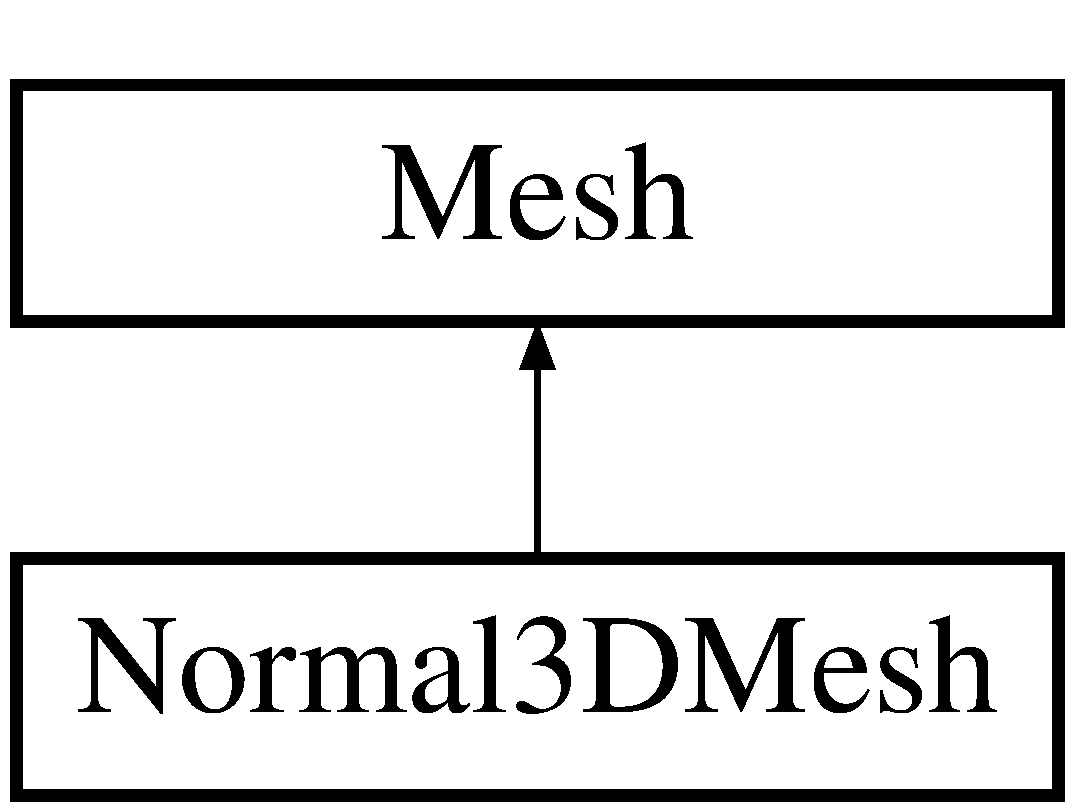
\includegraphics[height=2.000000cm]{class_normal3_d_mesh}
\end{center}
\end{figure}
\subsection*{Public Member Functions}
\begin{DoxyCompactItemize}
\item 
\hyperlink{class_normal3_d_mesh_a4eb05602fa8aa89dbfa135dd8b938055}{Normal3\+D\+Mesh} (Q\+File $\ast$obj\+Mesh\+File)
\item 
\hyperlink{class_normal3_d_mesh_aa596728d13cb7785a32fd18eb166a32c}{Normal3\+D\+Mesh} (Q\+String file)
\item 
\hyperlink{class_normal3_d_mesh_aa9d9e8bae673dca2b4b72666fdf6f4b4}{$\sim$\+Normal3\+D\+Mesh} ()
\end{DoxyCompactItemize}
\subsection*{Additional Inherited Members}


\subsection{Detailed Description}


Definition at line 7 of file normal3dmesh.\+h.



\subsection{Constructor \& Destructor Documentation}
\hypertarget{class_normal3_d_mesh_a4eb05602fa8aa89dbfa135dd8b938055}{}\index{Normal3\+D\+Mesh@{Normal3\+D\+Mesh}!Normal3\+D\+Mesh@{Normal3\+D\+Mesh}}
\index{Normal3\+D\+Mesh@{Normal3\+D\+Mesh}!Normal3\+D\+Mesh@{Normal3\+D\+Mesh}}
\subsubsection[{Normal3\+D\+Mesh(\+Q\+File $\ast$obj\+Mesh\+File)}]{\setlength{\rightskip}{0pt plus 5cm}Normal3\+D\+Mesh\+::\+Normal3\+D\+Mesh (
\begin{DoxyParamCaption}
\item[{Q\+File $\ast$}]{obj\+Mesh\+File}
\end{DoxyParamCaption}
)}\label{class_normal3_d_mesh_a4eb05602fa8aa89dbfa135dd8b938055}


Definition at line 98 of file normal3dmesh.\+cpp.

\hypertarget{class_normal3_d_mesh_aa596728d13cb7785a32fd18eb166a32c}{}\index{Normal3\+D\+Mesh@{Normal3\+D\+Mesh}!Normal3\+D\+Mesh@{Normal3\+D\+Mesh}}
\index{Normal3\+D\+Mesh@{Normal3\+D\+Mesh}!Normal3\+D\+Mesh@{Normal3\+D\+Mesh}}
\subsubsection[{Normal3\+D\+Mesh(\+Q\+String file)}]{\setlength{\rightskip}{0pt plus 5cm}Normal3\+D\+Mesh\+::\+Normal3\+D\+Mesh (
\begin{DoxyParamCaption}
\item[{Q\+String}]{file}
\end{DoxyParamCaption}
)}\label{class_normal3_d_mesh_aa596728d13cb7785a32fd18eb166a32c}


Definition at line 103 of file normal3dmesh.\+cpp.

\hypertarget{class_normal3_d_mesh_aa9d9e8bae673dca2b4b72666fdf6f4b4}{}\index{Normal3\+D\+Mesh@{Normal3\+D\+Mesh}!````~Normal3\+D\+Mesh@{$\sim$\+Normal3\+D\+Mesh}}
\index{````~Normal3\+D\+Mesh@{$\sim$\+Normal3\+D\+Mesh}!Normal3\+D\+Mesh@{Normal3\+D\+Mesh}}
\subsubsection[{$\sim$\+Normal3\+D\+Mesh()}]{\setlength{\rightskip}{0pt plus 5cm}Normal3\+D\+Mesh\+::$\sim$\+Normal3\+D\+Mesh (
\begin{DoxyParamCaption}
{}
\end{DoxyParamCaption}
)}\label{class_normal3_d_mesh_aa9d9e8bae673dca2b4b72666fdf6f4b4}


Definition at line 111 of file normal3dmesh.\+cpp.



The documentation for this class was generated from the following files\+:\begin{DoxyCompactItemize}
\item 
mesh/\hyperlink{normal3dmesh_8h}{normal3dmesh.\+h}\item 
mesh/\hyperlink{normal3dmesh_8cpp}{normal3dmesh.\+cpp}\end{DoxyCompactItemize}

\hypertarget{class_primitive_mesh}{}\section{Primitive\+Mesh Class Reference}
\label{class_primitive_mesh}\index{Primitive\+Mesh@{Primitive\+Mesh}}


{\ttfamily \#include $<$primitivemesh.\+h$>$}

Inheritance diagram for Primitive\+Mesh\+:\begin{figure}[H]
\begin{center}
\leavevmode
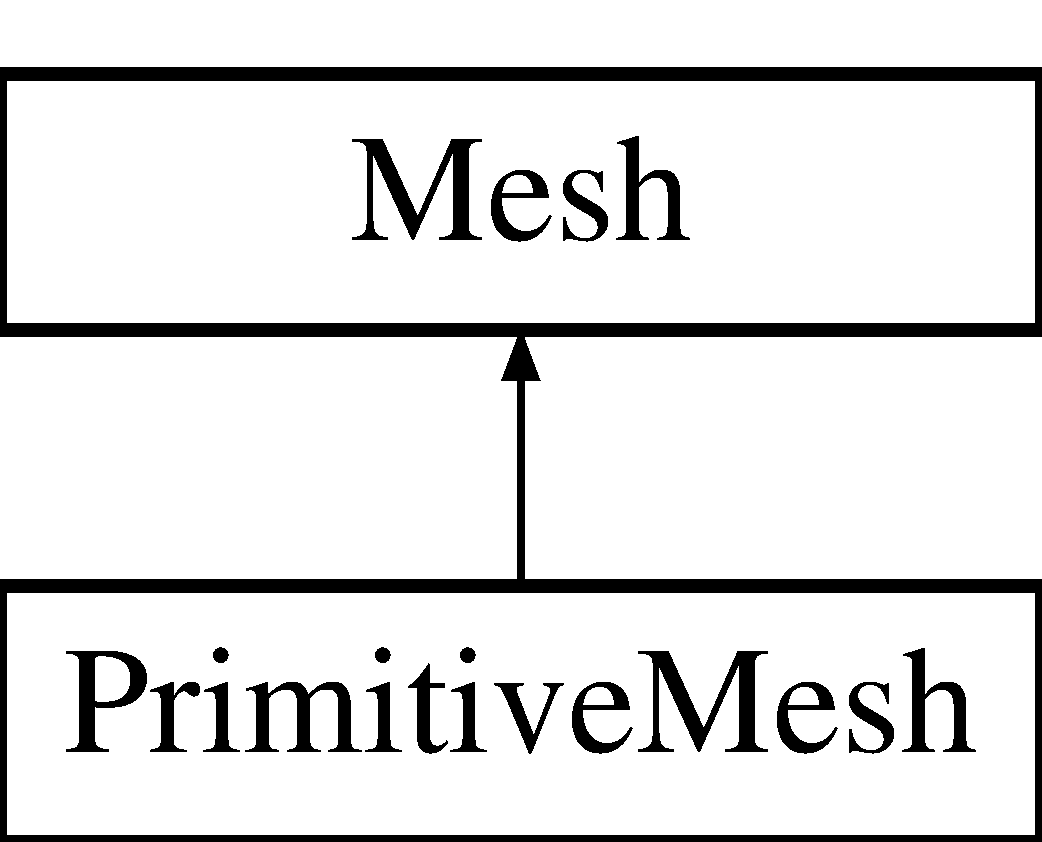
\includegraphics[height=2.000000cm]{class_primitive_mesh}
\end{center}
\end{figure}
\subsection*{Public Member Functions}
\begin{DoxyCompactItemize}
\item 
\hyperlink{class_primitive_mesh_a51ebe5f1c16753384ff2bf5ffd93063c}{Primitive\+Mesh} (\hyperlink{struct_shape_data}{Shape\+Data} $\ast$shape)
\item 
\hyperlink{class_primitive_mesh_abd454bdf8169c7e8b338ccaa341c3029}{$\sim$\+Primitive\+Mesh} ()
\end{DoxyCompactItemize}
\subsection*{Additional Inherited Members}


\subsection{Detailed Description}


Definition at line 8 of file primitivemesh.\+h.



\subsection{Constructor \& Destructor Documentation}
\hypertarget{class_primitive_mesh_a51ebe5f1c16753384ff2bf5ffd93063c}{}\index{Primitive\+Mesh@{Primitive\+Mesh}!Primitive\+Mesh@{Primitive\+Mesh}}
\index{Primitive\+Mesh@{Primitive\+Mesh}!Primitive\+Mesh@{Primitive\+Mesh}}
\subsubsection[{Primitive\+Mesh(\+Shape\+Data $\ast$shape)}]{\setlength{\rightskip}{0pt plus 5cm}Primitive\+Mesh\+::\+Primitive\+Mesh (
\begin{DoxyParamCaption}
\item[{{\bf Shape\+Data} $\ast$}]{shape}
\end{DoxyParamCaption}
)}\label{class_primitive_mesh_a51ebe5f1c16753384ff2bf5ffd93063c}


Definition at line 3 of file primitivemesh.\+cpp.

\hypertarget{class_primitive_mesh_abd454bdf8169c7e8b338ccaa341c3029}{}\index{Primitive\+Mesh@{Primitive\+Mesh}!````~Primitive\+Mesh@{$\sim$\+Primitive\+Mesh}}
\index{````~Primitive\+Mesh@{$\sim$\+Primitive\+Mesh}!Primitive\+Mesh@{Primitive\+Mesh}}
\subsubsection[{$\sim$\+Primitive\+Mesh()}]{\setlength{\rightskip}{0pt plus 5cm}Primitive\+Mesh\+::$\sim$\+Primitive\+Mesh (
\begin{DoxyParamCaption}
{}
\end{DoxyParamCaption}
)}\label{class_primitive_mesh_abd454bdf8169c7e8b338ccaa341c3029}


Definition at line 30 of file primitivemesh.\+cpp.



The documentation for this class was generated from the following files\+:\begin{DoxyCompactItemize}
\item 
mesh/\hyperlink{primitivemesh_8h}{primitivemesh.\+h}\item 
mesh/\hyperlink{primitivemesh_8cpp}{primitivemesh.\+cpp}\end{DoxyCompactItemize}

\hypertarget{class_renderable}{}\section{Renderable Class Reference}
\label{class_renderable}\index{Renderable@{Renderable}}


The \{abstract\} \hyperlink{class_renderable}{Renderable} class.  




{\ttfamily \#include $<$renderable.\+h$>$}

Inheritance diagram for Renderable\+:\begin{figure}[H]
\begin{center}
\leavevmode
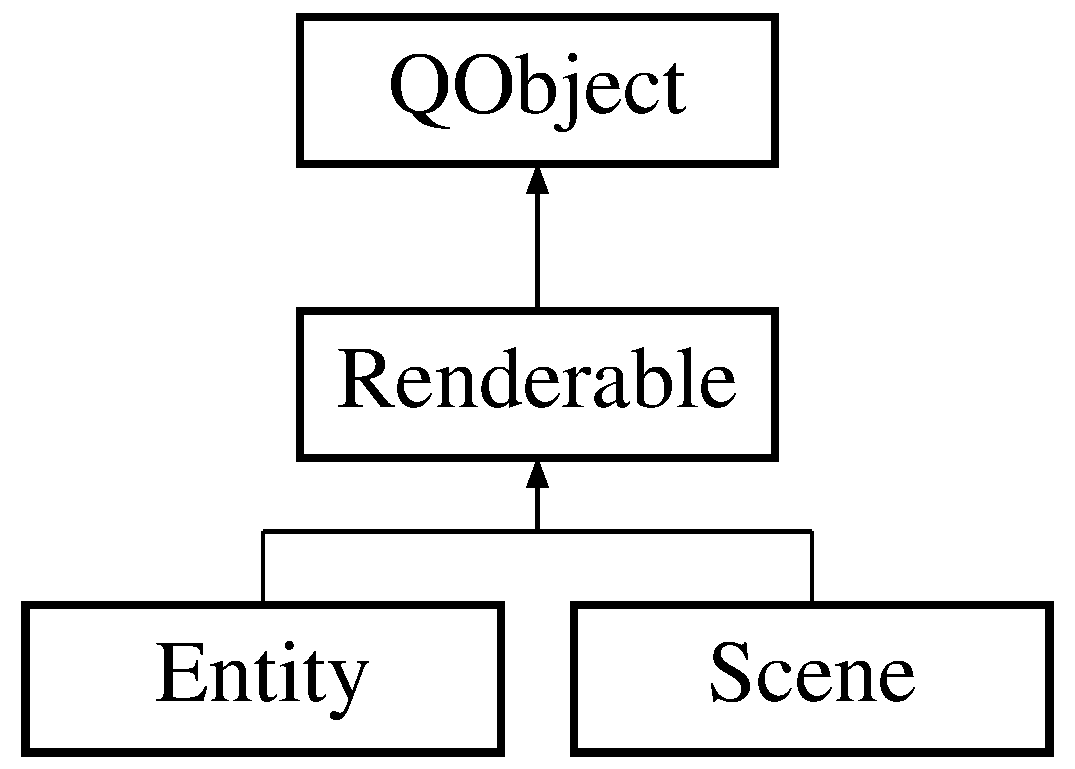
\includegraphics[height=3.000000cm]{class_renderable}
\end{center}
\end{figure}
\subsection*{Public Member Functions}
\begin{DoxyCompactItemize}
\item 
\hyperlink{class_renderable_aec20cb09808c028d3d024e02b86e0272}{Renderable} (Q\+Open\+G\+L\+Context $\ast$context, const Q\+Matrix4x4 $\ast$p\+World, const Q\+String str\+Name=\char`\"{}Renderable\char`\"{}, Q\+Object $\ast$parent=0)
\item 
virtual \hyperlink{class_renderable_a4c9e03ac345df99a010c2ad9f8632af2}{$\sim$\+Renderable} ()
\item 
virtual void \hyperlink{class_renderable_ab204246b39a34b14a3f258a065cc3019}{Create} ()=0
\begin{DoxyCompactList}\small\item\em Create. \end{DoxyCompactList}\item 
virtual void \hyperlink{class_renderable_aaf8e0b324e35f8a1b61a9667a0d91d51}{Destroy} ()=0
\begin{DoxyCompactList}\small\item\em Destroy. \end{DoxyCompactList}\item 
virtual void \hyperlink{class_renderable_aee9a55d459edefe6c8b8532ab5d7102c}{Render} (G\+Luint draw\+Order, const Q\+Matrix4x4 $\ast$p\+View, const Q\+Matrix4x4 $\ast$p\+Proj, const \hyperlink{class_light}{Light} $\ast$p\+Light)=0
\begin{DoxyCompactList}\small\item\em Render renders the object to the open\+Gl contex. \end{DoxyCompactList}\item 
virtual void \hyperlink{class_renderable_ac3bc83ee89ef2a6523277ba74fdcf0a8}{update} (double f\+Time, double f\+Elapsed\+Time)
\begin{DoxyCompactList}\small\item\em update an animated Renerable Object \end{DoxyCompactList}\item 
virtual Q\+Matrix4x4 $\ast$ \hyperlink{class_renderable_ac2098bbc9937aff7099d36c6b425c2a2}{get\+World\+Matrix} ()
\item 
virtual void \hyperlink{class_renderable_ad5f7e6f7ef8e555be642c1e311656b45}{set\+World\+Matrix} (const Q\+Matrix4x4 \&n\+World)
\item 
Q\+String \hyperlink{class_renderable_a844b90c20cad45b553390cfed94f4517}{get\+Name} ()
\item 
void \hyperlink{class_renderable_a772b6d4edbff1d75922dab9476828bb5}{set\+Name} (Q\+String n\+Name)
\end{DoxyCompactItemize}
\subsection*{Protected Attributes}
\begin{DoxyCompactItemize}
\item 
Q\+Open\+G\+L\+Context $\ast$ \hyperlink{class_renderable_a16e9fd9850fd35318e3c215bbd4ceb50}{context\+Device}
\item 
Q\+Matrix4x4 $\ast$ \hyperlink{class_renderable_ac0aa4963b49ad1b2b21affc08f733f00}{mat\+World}
\item 
Q\+String \hyperlink{class_renderable_a09b50e8371e55294da5a383475c53783}{name}
\end{DoxyCompactItemize}


\subsection{Detailed Description}
The \{abstract\} \hyperlink{class_renderable}{Renderable} class. 

abstract class for an Object that is renderable with open\+G\+L

\hyperlink{class_renderable_ab204246b39a34b14a3f258a065cc3019}{Create()}, \hyperlink{class_renderable_aaf8e0b324e35f8a1b61a9667a0d91d51}{Destroy()}, \hyperlink{class_renderable_aee9a55d459edefe6c8b8532ab5d7102c}{Render()} and \hyperlink{class_renderable_ac3bc83ee89ef2a6523277ba74fdcf0a8}{update()} needs at least to be implemented 

Definition at line 15 of file renderable.\+h.



\subsection{Constructor \& Destructor Documentation}
\hypertarget{class_renderable_aec20cb09808c028d3d024e02b86e0272}{}\index{Renderable@{Renderable}!Renderable@{Renderable}}
\index{Renderable@{Renderable}!Renderable@{Renderable}}
\subsubsection[{Renderable(\+Q\+Open\+G\+L\+Context $\ast$context, const Q\+Matrix4x4 $\ast$p\+World, const Q\+String str\+Name=""Renderable"", Q\+Object $\ast$parent=0)}]{\setlength{\rightskip}{0pt plus 5cm}Renderable\+::\+Renderable (
\begin{DoxyParamCaption}
\item[{Q\+Open\+G\+L\+Context $\ast$}]{context, }
\item[{const Q\+Matrix4x4 $\ast$}]{p\+World, }
\item[{const Q\+String}]{str\+Name = {\ttfamily \char`\"{}Renderable\char`\"{}}, }
\item[{Q\+Object $\ast$}]{parent = {\ttfamily 0}}
\end{DoxyParamCaption}
)\hspace{0.3cm}{\ttfamily [explicit]}}\label{class_renderable_aec20cb09808c028d3d024e02b86e0272}


Definition at line 3 of file renderable.\+cpp.

\hypertarget{class_renderable_a4c9e03ac345df99a010c2ad9f8632af2}{}\index{Renderable@{Renderable}!````~Renderable@{$\sim$\+Renderable}}
\index{````~Renderable@{$\sim$\+Renderable}!Renderable@{Renderable}}
\subsubsection[{$\sim$\+Renderable()}]{\setlength{\rightskip}{0pt plus 5cm}virtual Renderable\+::$\sim$\+Renderable (
\begin{DoxyParamCaption}
{}
\end{DoxyParamCaption}
)\hspace{0.3cm}{\ttfamily [inline]}, {\ttfamily [virtual]}}\label{class_renderable_a4c9e03ac345df99a010c2ad9f8632af2}


Definition at line 28 of file renderable.\+h.



\subsection{Member Function Documentation}
\hypertarget{class_renderable_ab204246b39a34b14a3f258a065cc3019}{}\index{Renderable@{Renderable}!Create@{Create}}
\index{Create@{Create}!Renderable@{Renderable}}
\subsubsection[{Create()=0}]{\setlength{\rightskip}{0pt plus 5cm}virtual void Renderable\+::\+Create (
\begin{DoxyParamCaption}
{}
\end{DoxyParamCaption}
)\hspace{0.3cm}{\ttfamily [pure virtual]}}\label{class_renderable_ab204246b39a34b14a3f258a065cc3019}


Create. 

Creates the \hyperlink{class_renderable}{Renderable} and initialize all open\+G\+L values 

Implemented in \hyperlink{class_entity_a647d154620c6464168f3b088f0ac170e}{Entity}, and \hyperlink{class_scene_a3a16f308d18a168f7778b9c3a29b3ac5}{Scene}.

\hypertarget{class_renderable_aaf8e0b324e35f8a1b61a9667a0d91d51}{}\index{Renderable@{Renderable}!Destroy@{Destroy}}
\index{Destroy@{Destroy}!Renderable@{Renderable}}
\subsubsection[{Destroy()=0}]{\setlength{\rightskip}{0pt plus 5cm}virtual void Renderable\+::\+Destroy (
\begin{DoxyParamCaption}
{}
\end{DoxyParamCaption}
)\hspace{0.3cm}{\ttfamily [pure virtual]}}\label{class_renderable_aaf8e0b324e35f8a1b61a9667a0d91d51}


Destroy. 

Destroies the \hyperlink{class_renderable}{Renderable} 

Implemented in \hyperlink{class_entity_aa75151fc607686b42d27f8c3ba73143d}{Entity}, and \hyperlink{class_scene_ac8261e2bf3f39d17c921f0ccbfb1f48f}{Scene}.

\hypertarget{class_renderable_a844b90c20cad45b553390cfed94f4517}{}\index{Renderable@{Renderable}!get\+Name@{get\+Name}}
\index{get\+Name@{get\+Name}!Renderable@{Renderable}}
\subsubsection[{get\+Name()}]{\setlength{\rightskip}{0pt plus 5cm}Q\+String Renderable\+::get\+Name (
\begin{DoxyParamCaption}
{}
\end{DoxyParamCaption}
)\hspace{0.3cm}{\ttfamily [inline]}}\label{class_renderable_a844b90c20cad45b553390cfed94f4517}


Definition at line 65 of file renderable.\+h.

\hypertarget{class_renderable_ac2098bbc9937aff7099d36c6b425c2a2}{}\index{Renderable@{Renderable}!get\+World\+Matrix@{get\+World\+Matrix}}
\index{get\+World\+Matrix@{get\+World\+Matrix}!Renderable@{Renderable}}
\subsubsection[{get\+World\+Matrix()}]{\setlength{\rightskip}{0pt plus 5cm}Q\+Matrix4x4 $\ast$ Renderable\+::get\+World\+Matrix (
\begin{DoxyParamCaption}
{}
\end{DoxyParamCaption}
)\hspace{0.3cm}{\ttfamily [virtual]}}\label{class_renderable_ac2098bbc9937aff7099d36c6b425c2a2}


Definition at line 12 of file renderable.\+cpp.

\hypertarget{class_renderable_aee9a55d459edefe6c8b8532ab5d7102c}{}\index{Renderable@{Renderable}!Render@{Render}}
\index{Render@{Render}!Renderable@{Renderable}}
\subsubsection[{Render(\+G\+Luint draw\+Order, const Q\+Matrix4x4 $\ast$p\+View, const Q\+Matrix4x4 $\ast$p\+Proj, const Light $\ast$p\+Light)=0}]{\setlength{\rightskip}{0pt plus 5cm}virtual void Renderable\+::\+Render (
\begin{DoxyParamCaption}
\item[{G\+Luint}]{draw\+Order, }
\item[{const Q\+Matrix4x4 $\ast$}]{p\+View, }
\item[{const Q\+Matrix4x4 $\ast$}]{p\+Proj, }
\item[{const {\bf Light} $\ast$}]{p\+Light}
\end{DoxyParamCaption}
)\hspace{0.3cm}{\ttfamily [pure virtual]}}\label{class_renderable_aee9a55d459edefe6c8b8532ab5d7102c}


Render renders the object to the open\+Gl contex. 


\begin{DoxyParams}{Parameters}
{\em draw\+Order} & \\
\hline
{\em p\+View} & Q\+Matrix4x4\}$\ast$ view matrix; \\
\hline
{\em p\+Proj} & Q\+Matrix4x4\mbox{]}$\ast$ projection matrix \\
\hline
\end{DoxyParams}


Implemented in \hyperlink{class_entity_a0f3f11bbb868ab96e5bbb0f835eb9966}{Entity}, and \hyperlink{class_scene_a61d176e58a0cf69bb201b3ac052ba84e}{Scene}.

\hypertarget{class_renderable_a772b6d4edbff1d75922dab9476828bb5}{}\index{Renderable@{Renderable}!set\+Name@{set\+Name}}
\index{set\+Name@{set\+Name}!Renderable@{Renderable}}
\subsubsection[{set\+Name(\+Q\+String n\+Name)}]{\setlength{\rightskip}{0pt plus 5cm}void Renderable\+::set\+Name (
\begin{DoxyParamCaption}
\item[{Q\+String}]{n\+Name}
\end{DoxyParamCaption}
)\hspace{0.3cm}{\ttfamily [inline]}}\label{class_renderable_a772b6d4edbff1d75922dab9476828bb5}


Definition at line 66 of file renderable.\+h.

\hypertarget{class_renderable_ad5f7e6f7ef8e555be642c1e311656b45}{}\index{Renderable@{Renderable}!set\+World\+Matrix@{set\+World\+Matrix}}
\index{set\+World\+Matrix@{set\+World\+Matrix}!Renderable@{Renderable}}
\subsubsection[{set\+World\+Matrix(const Q\+Matrix4x4 \&n\+World)}]{\setlength{\rightskip}{0pt plus 5cm}void Renderable\+::set\+World\+Matrix (
\begin{DoxyParamCaption}
\item[{const Q\+Matrix4x4 \&}]{n\+World}
\end{DoxyParamCaption}
)\hspace{0.3cm}{\ttfamily [virtual]}}\label{class_renderable_ad5f7e6f7ef8e555be642c1e311656b45}


Definition at line 17 of file renderable.\+cpp.

\hypertarget{class_renderable_ac3bc83ee89ef2a6523277ba74fdcf0a8}{}\index{Renderable@{Renderable}!update@{update}}
\index{update@{update}!Renderable@{Renderable}}
\subsubsection[{update(double f\+Time, double f\+Elapsed\+Time)}]{\setlength{\rightskip}{0pt plus 5cm}virtual void Renderable\+::update (
\begin{DoxyParamCaption}
\item[{double}]{f\+Time, }
\item[{double}]{f\+Elapsed\+Time}
\end{DoxyParamCaption}
)\hspace{0.3cm}{\ttfamily [inline]}, {\ttfamily [virtual]}}\label{class_renderable_ac3bc83ee89ef2a6523277ba74fdcf0a8}


update an animated Renerable Object 


\begin{DoxyParams}{Parameters}
{\em f\+Time} & \\
\hline
{\em f\+Elapsed\+Time} & \\
\hline
\end{DoxyParams}


Definition at line 60 of file renderable.\+h.



\subsection{Member Data Documentation}
\hypertarget{class_renderable_a16e9fd9850fd35318e3c215bbd4ceb50}{}\index{Renderable@{Renderable}!context\+Device@{context\+Device}}
\index{context\+Device@{context\+Device}!Renderable@{Renderable}}
\subsubsection[{context\+Device}]{\setlength{\rightskip}{0pt plus 5cm}Q\+Open\+G\+L\+Context$\ast$ Renderable\+::context\+Device\hspace{0.3cm}{\ttfamily [protected]}}\label{class_renderable_a16e9fd9850fd35318e3c215bbd4ceb50}


Definition at line 19 of file renderable.\+h.

\hypertarget{class_renderable_ac0aa4963b49ad1b2b21affc08f733f00}{}\index{Renderable@{Renderable}!mat\+World@{mat\+World}}
\index{mat\+World@{mat\+World}!Renderable@{Renderable}}
\subsubsection[{mat\+World}]{\setlength{\rightskip}{0pt plus 5cm}Q\+Matrix4x4$\ast$ Renderable\+::mat\+World\hspace{0.3cm}{\ttfamily [protected]}}\label{class_renderable_ac0aa4963b49ad1b2b21affc08f733f00}


Definition at line 20 of file renderable.\+h.

\hypertarget{class_renderable_a09b50e8371e55294da5a383475c53783}{}\index{Renderable@{Renderable}!name@{name}}
\index{name@{name}!Renderable@{Renderable}}
\subsubsection[{name}]{\setlength{\rightskip}{0pt plus 5cm}Q\+String Renderable\+::name\hspace{0.3cm}{\ttfamily [protected]}}\label{class_renderable_a09b50e8371e55294da5a383475c53783}


Definition at line 22 of file renderable.\+h.



The documentation for this class was generated from the following files\+:\begin{DoxyCompactItemize}
\item 
\hyperlink{renderable_8h}{renderable.\+h}\item 
\hyperlink{renderable_8cpp}{renderable.\+cpp}\end{DoxyCompactItemize}

\hypertarget{class_scene}{}\section{Scene Class Reference}
\label{class_scene}\index{Scene@{Scene}}


The \hyperlink{class_scene}{Scene} class.  




{\ttfamily \#include $<$scene.\+h$>$}

Inheritance diagram for Scene\+:\begin{figure}[H]
\begin{center}
\leavevmode
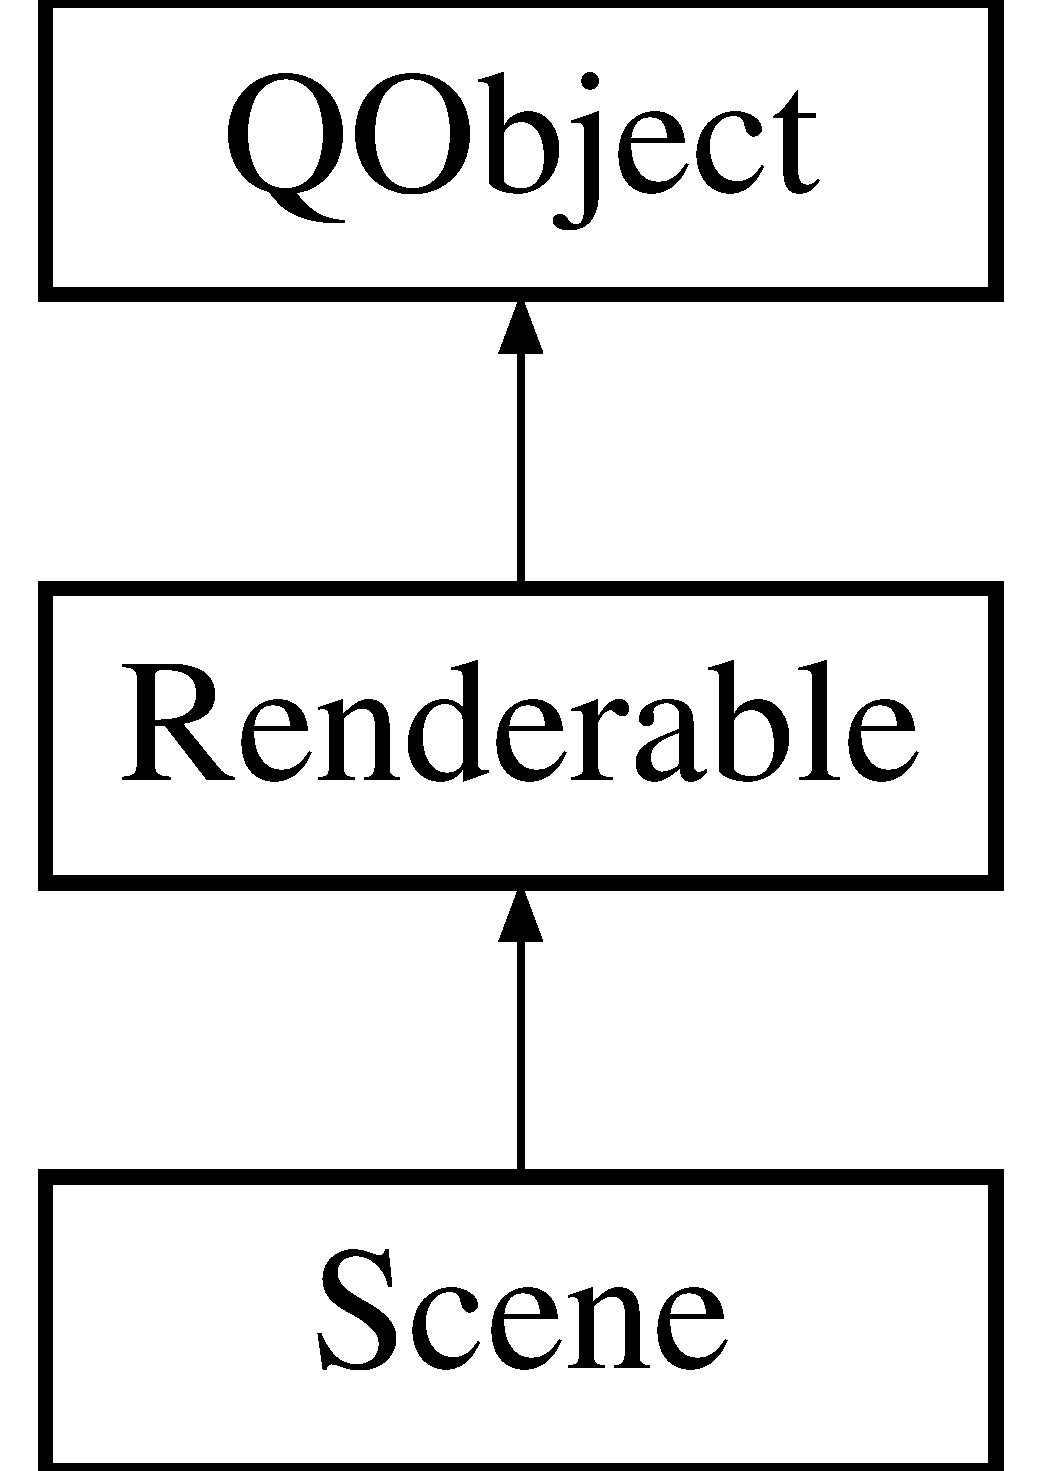
\includegraphics[height=3.000000cm]{class_scene}
\end{center}
\end{figure}
\subsection*{Public Member Functions}
\begin{DoxyCompactItemize}
\item 
\hyperlink{class_scene_a209847445cd18171aeae4a1a7637efea}{Scene} (Q\+Open\+G\+L\+Context $\ast$context, Q\+Object $\ast$parent=0)
\item 
\hyperlink{class_scene_a3b8cec2e32546713915f8c6303c951f1}{$\sim$\+Scene} ()
\item 
void \hyperlink{class_scene_a99ecb7628446690510dd1bb27dffc8e5}{add\+Material} (\hyperlink{class_material}{Material} $\ast$material)
\item 
void \hyperlink{class_scene_ac9add8bc84e2fcf26fede56e1d40a8ff}{remove\+Material} (\hyperlink{class_material}{Material} $\ast$material)
\item 
void \hyperlink{class_scene_a14884548876ba098f476afa0a4c6c030}{remove\+Material} (int at)
\item 
void \hyperlink{class_scene_a621e3f935f8bec1fa2d6b29eeeda8eaa}{add\+Renderable} (\hyperlink{class_renderable}{Renderable} $\ast$object)
\item 
void \hyperlink{class_scene_a585aebb726cb8a3ceca6cc8189e7bcd7}{remove\+Renderable} (int at)
\item 
void \hyperlink{class_scene_a161f58ff37be2425a9d716e73ba8d3b3}{remove\+Renderable} (\hyperlink{class_renderable}{Renderable} $\ast$object)
\item 
\hyperlink{class_camera}{Camera} $\ast$ \hyperlink{class_scene_a1845161fcd088622a1288a6c41bcd574}{camera} ()
\item 
\hyperlink{class_light}{Light} $\ast$ \hyperlink{class_scene_a01d2124c572f0341cb317745d3b7a0a4}{light} ()
\item 
virtual void \hyperlink{class_scene_a3a16f308d18a168f7778b9c3a29b3ac5}{Create} ()
\begin{DoxyCompactList}\small\item\em Create. \end{DoxyCompactList}\item 
virtual void \hyperlink{class_scene_ac8261e2bf3f39d17c921f0ccbfb1f48f}{Destroy} ()
\begin{DoxyCompactList}\small\item\em Destroy. \end{DoxyCompactList}\item 
virtual void \hyperlink{class_scene_a61d176e58a0cf69bb201b3ac052ba84e}{Render} (G\+Luint draw\+Order, const Q\+Matrix4x4 $\ast$p\+View, const Q\+Matrix4x4 $\ast$p\+Proj, const \hyperlink{class_light}{Light} $\ast$p\+Light)
\begin{DoxyCompactList}\small\item\em Render renders the object to the open\+Gl contex. \end{DoxyCompactList}\item 
void \hyperlink{class_scene_a91913b921d41d374e00eac347358dc14}{Render} ()
\end{DoxyCompactItemize}
\subsection*{Additional Inherited Members}


\subsection{Detailed Description}
The \hyperlink{class_scene}{Scene} class. 

Describes a \hyperlink{class_scene}{Scene} of renderable Objects and holds dem in a Layer togehtner 

Definition at line 19 of file scene.\+h.



\subsection{Constructor \& Destructor Documentation}
\hypertarget{class_scene_a209847445cd18171aeae4a1a7637efea}{}\index{Scene@{Scene}!Scene@{Scene}}
\index{Scene@{Scene}!Scene@{Scene}}
\subsubsection[{Scene(\+Q\+Open\+G\+L\+Context $\ast$context, Q\+Object $\ast$parent=0)}]{\setlength{\rightskip}{0pt plus 5cm}Scene\+::\+Scene (
\begin{DoxyParamCaption}
\item[{Q\+Open\+G\+L\+Context $\ast$}]{context, }
\item[{Q\+Object $\ast$}]{parent = {\ttfamily 0}}
\end{DoxyParamCaption}
)\hspace{0.3cm}{\ttfamily [explicit]}}\label{class_scene_a209847445cd18171aeae4a1a7637efea}


Definition at line 3 of file scene.\+cpp.

\hypertarget{class_scene_a3b8cec2e32546713915f8c6303c951f1}{}\index{Scene@{Scene}!````~Scene@{$\sim$\+Scene}}
\index{````~Scene@{$\sim$\+Scene}!Scene@{Scene}}
\subsubsection[{$\sim$\+Scene()}]{\setlength{\rightskip}{0pt plus 5cm}Scene\+::$\sim$\+Scene (
\begin{DoxyParamCaption}
{}
\end{DoxyParamCaption}
)}\label{class_scene_a3b8cec2e32546713915f8c6303c951f1}


Definition at line 9 of file scene.\+cpp.



\subsection{Member Function Documentation}
\hypertarget{class_scene_a99ecb7628446690510dd1bb27dffc8e5}{}\index{Scene@{Scene}!add\+Material@{add\+Material}}
\index{add\+Material@{add\+Material}!Scene@{Scene}}
\subsubsection[{add\+Material(\+Material $\ast$material)}]{\setlength{\rightskip}{0pt plus 5cm}void Scene\+::add\+Material (
\begin{DoxyParamCaption}
\item[{{\bf Material} $\ast$}]{material}
\end{DoxyParamCaption}
)}\label{class_scene_a99ecb7628446690510dd1bb27dffc8e5}


Definition at line 15 of file scene.\+cpp.

\hypertarget{class_scene_a621e3f935f8bec1fa2d6b29eeeda8eaa}{}\index{Scene@{Scene}!add\+Renderable@{add\+Renderable}}
\index{add\+Renderable@{add\+Renderable}!Scene@{Scene}}
\subsubsection[{add\+Renderable(\+Renderable $\ast$object)}]{\setlength{\rightskip}{0pt plus 5cm}void Scene\+::add\+Renderable (
\begin{DoxyParamCaption}
\item[{{\bf Renderable} $\ast$}]{object}
\end{DoxyParamCaption}
)}\label{class_scene_a621e3f935f8bec1fa2d6b29eeeda8eaa}


Definition at line 20 of file scene.\+cpp.

\hypertarget{class_scene_a1845161fcd088622a1288a6c41bcd574}{}\index{Scene@{Scene}!camera@{camera}}
\index{camera@{camera}!Scene@{Scene}}
\subsubsection[{camera()}]{\setlength{\rightskip}{0pt plus 5cm}{\bf Camera}$\ast$ Scene\+::camera (
\begin{DoxyParamCaption}
{}
\end{DoxyParamCaption}
)\hspace{0.3cm}{\ttfamily [inline]}}\label{class_scene_a1845161fcd088622a1288a6c41bcd574}


Definition at line 40 of file scene.\+h.

\hypertarget{class_scene_a3a16f308d18a168f7778b9c3a29b3ac5}{}\index{Scene@{Scene}!Create@{Create}}
\index{Create@{Create}!Scene@{Scene}}
\subsubsection[{Create()}]{\setlength{\rightskip}{0pt plus 5cm}void Scene\+::\+Create (
\begin{DoxyParamCaption}
{}
\end{DoxyParamCaption}
)\hspace{0.3cm}{\ttfamily [virtual]}}\label{class_scene_a3a16f308d18a168f7778b9c3a29b3ac5}


Create. 

Creates the \hyperlink{class_renderable}{Renderable} and initialize all open\+G\+L values 

Implements \hyperlink{class_renderable_ab204246b39a34b14a3f258a065cc3019}{Renderable}.



Definition at line 39 of file scene.\+cpp.

\hypertarget{class_scene_ac8261e2bf3f39d17c921f0ccbfb1f48f}{}\index{Scene@{Scene}!Destroy@{Destroy}}
\index{Destroy@{Destroy}!Scene@{Scene}}
\subsubsection[{Destroy()}]{\setlength{\rightskip}{0pt plus 5cm}void Scene\+::\+Destroy (
\begin{DoxyParamCaption}
{}
\end{DoxyParamCaption}
)\hspace{0.3cm}{\ttfamily [virtual]}}\label{class_scene_ac8261e2bf3f39d17c921f0ccbfb1f48f}


Destroy. 

Destroies the \hyperlink{class_renderable}{Renderable} 

Implements \hyperlink{class_renderable_aaf8e0b324e35f8a1b61a9667a0d91d51}{Renderable}.



Definition at line 46 of file scene.\+cpp.

\hypertarget{class_scene_a01d2124c572f0341cb317745d3b7a0a4}{}\index{Scene@{Scene}!light@{light}}
\index{light@{light}!Scene@{Scene}}
\subsubsection[{light()}]{\setlength{\rightskip}{0pt plus 5cm}{\bf Light}$\ast$ Scene\+::light (
\begin{DoxyParamCaption}
{}
\end{DoxyParamCaption}
)\hspace{0.3cm}{\ttfamily [inline]}}\label{class_scene_a01d2124c572f0341cb317745d3b7a0a4}


Definition at line 41 of file scene.\+h.

\hypertarget{class_scene_ac9add8bc84e2fcf26fede56e1d40a8ff}{}\index{Scene@{Scene}!remove\+Material@{remove\+Material}}
\index{remove\+Material@{remove\+Material}!Scene@{Scene}}
\subsubsection[{remove\+Material(\+Material $\ast$material)}]{\setlength{\rightskip}{0pt plus 5cm}void Scene\+::remove\+Material (
\begin{DoxyParamCaption}
\item[{{\bf Material} $\ast$}]{material}
\end{DoxyParamCaption}
)}\label{class_scene_ac9add8bc84e2fcf26fede56e1d40a8ff}
\hypertarget{class_scene_a14884548876ba098f476afa0a4c6c030}{}\index{Scene@{Scene}!remove\+Material@{remove\+Material}}
\index{remove\+Material@{remove\+Material}!Scene@{Scene}}
\subsubsection[{remove\+Material(int at)}]{\setlength{\rightskip}{0pt plus 5cm}void Scene\+::remove\+Material (
\begin{DoxyParamCaption}
\item[{int}]{at}
\end{DoxyParamCaption}
)}\label{class_scene_a14884548876ba098f476afa0a4c6c030}
\hypertarget{class_scene_a585aebb726cb8a3ceca6cc8189e7bcd7}{}\index{Scene@{Scene}!remove\+Renderable@{remove\+Renderable}}
\index{remove\+Renderable@{remove\+Renderable}!Scene@{Scene}}
\subsubsection[{remove\+Renderable(int at)}]{\setlength{\rightskip}{0pt plus 5cm}void Scene\+::remove\+Renderable (
\begin{DoxyParamCaption}
\item[{int}]{at}
\end{DoxyParamCaption}
)}\label{class_scene_a585aebb726cb8a3ceca6cc8189e7bcd7}
\hypertarget{class_scene_a161f58ff37be2425a9d716e73ba8d3b3}{}\index{Scene@{Scene}!remove\+Renderable@{remove\+Renderable}}
\index{remove\+Renderable@{remove\+Renderable}!Scene@{Scene}}
\subsubsection[{remove\+Renderable(\+Renderable $\ast$object)}]{\setlength{\rightskip}{0pt plus 5cm}void Scene\+::remove\+Renderable (
\begin{DoxyParamCaption}
\item[{{\bf Renderable} $\ast$}]{object}
\end{DoxyParamCaption}
)}\label{class_scene_a161f58ff37be2425a9d716e73ba8d3b3}
\hypertarget{class_scene_a61d176e58a0cf69bb201b3ac052ba84e}{}\index{Scene@{Scene}!Render@{Render}}
\index{Render@{Render}!Scene@{Scene}}
\subsubsection[{Render(\+G\+Luint draw\+Order, const Q\+Matrix4x4 $\ast$p\+View, const Q\+Matrix4x4 $\ast$p\+Proj, const Light $\ast$p\+Light)}]{\setlength{\rightskip}{0pt plus 5cm}void Scene\+::\+Render (
\begin{DoxyParamCaption}
\item[{G\+Luint}]{draw\+Order, }
\item[{const Q\+Matrix4x4 $\ast$}]{p\+View, }
\item[{const Q\+Matrix4x4 $\ast$}]{p\+Proj, }
\item[{const {\bf Light} $\ast$}]{p\+Light}
\end{DoxyParamCaption}
)\hspace{0.3cm}{\ttfamily [virtual]}}\label{class_scene_a61d176e58a0cf69bb201b3ac052ba84e}


Render renders the object to the open\+Gl contex. 


\begin{DoxyParams}{Parameters}
{\em draw\+Order} & \\
\hline
{\em p\+View} & Q\+Matrix4x4\}$\ast$ view matrix; \\
\hline
{\em p\+Proj} & Q\+Matrix4x4\mbox{]}$\ast$ projection matrix \\
\hline
\end{DoxyParams}


Implements \hyperlink{class_renderable_aee9a55d459edefe6c8b8532ab5d7102c}{Renderable}.



Definition at line 25 of file scene.\+cpp.

\hypertarget{class_scene_a91913b921d41d374e00eac347358dc14}{}\index{Scene@{Scene}!Render@{Render}}
\index{Render@{Render}!Scene@{Scene}}
\subsubsection[{Render()}]{\setlength{\rightskip}{0pt plus 5cm}void Scene\+::\+Render (
\begin{DoxyParamCaption}
{}
\end{DoxyParamCaption}
)}\label{class_scene_a91913b921d41d374e00eac347358dc14}


Definition at line 63 of file scene.\+cpp.



The documentation for this class was generated from the following files\+:\begin{DoxyCompactItemize}
\item 
\hyperlink{scene_8h}{scene.\+h}\item 
\hyperlink{scene_8cpp}{scene.\+cpp}\end{DoxyCompactItemize}

\hypertarget{struct_shape_data}{}\section{Shape\+Data Struct Reference}
\label{struct_shape_data}\index{Shape\+Data@{Shape\+Data}}


{\ttfamily \#include $<$shapedata.\+h$>$}

\subsection*{Public Member Functions}
\begin{DoxyCompactItemize}
\item 
\hyperlink{struct_shape_data_a76d5ff4056efb0a5703793ef55b06651}{Shape\+Data} ()
\item 
G\+Lsizeiptr \hyperlink{struct_shape_data_a5b838f3fc07c63aeb718b8c22bc3e2cb}{vertex\+Buffer\+Size} () const 
\item 
G\+Lsizeiptr \hyperlink{struct_shape_data_afa0a214679b4acbf5a8e38d10ef48779}{index\+Buffer\+Size} () const 
\item 
void \hyperlink{struct_shape_data_a59e005d5410ad30435357d385e73ef48}{cleanup} ()
\end{DoxyCompactItemize}
\subsection*{Public Attributes}
\begin{DoxyCompactItemize}
\item 
\hyperlink{class_vertex}{Vertex} $\ast$ \hyperlink{struct_shape_data_a4cb9087cff7d75dcba0cc6acf363468b}{vertices}
\item 
G\+Luint \hyperlink{struct_shape_data_a255bf343d438b66c7a5a59f9c2a9be07}{num\+Vertices}
\item 
G\+Lushort $\ast$ \hyperlink{struct_shape_data_ab2814a4ce1455f39db59b819b62fd44e}{indices}
\item 
G\+Luint \hyperlink{struct_shape_data_ab4ef69f08567dec90213e8a204afb6ff}{num\+Indices}
\end{DoxyCompactItemize}


\subsection{Detailed Description}


Definition at line 6 of file shapedata.\+h.



\subsection{Constructor \& Destructor Documentation}
\hypertarget{struct_shape_data_a76d5ff4056efb0a5703793ef55b06651}{}\index{Shape\+Data@{Shape\+Data}!Shape\+Data@{Shape\+Data}}
\index{Shape\+Data@{Shape\+Data}!Shape\+Data@{Shape\+Data}}
\subsubsection[{Shape\+Data()}]{\setlength{\rightskip}{0pt plus 5cm}Shape\+Data\+::\+Shape\+Data (
\begin{DoxyParamCaption}
{}
\end{DoxyParamCaption}
)\hspace{0.3cm}{\ttfamily [inline]}}\label{struct_shape_data_a76d5ff4056efb0a5703793ef55b06651}


Definition at line 8 of file shapedata.\+h.



\subsection{Member Function Documentation}
\hypertarget{struct_shape_data_a59e005d5410ad30435357d385e73ef48}{}\index{Shape\+Data@{Shape\+Data}!cleanup@{cleanup}}
\index{cleanup@{cleanup}!Shape\+Data@{Shape\+Data}}
\subsubsection[{cleanup()}]{\setlength{\rightskip}{0pt plus 5cm}void Shape\+Data\+::cleanup (
\begin{DoxyParamCaption}
{}
\end{DoxyParamCaption}
)\hspace{0.3cm}{\ttfamily [inline]}}\label{struct_shape_data_a59e005d5410ad30435357d385e73ef48}


Definition at line 25 of file shapedata.\+h.

\hypertarget{struct_shape_data_afa0a214679b4acbf5a8e38d10ef48779}{}\index{Shape\+Data@{Shape\+Data}!index\+Buffer\+Size@{index\+Buffer\+Size}}
\index{index\+Buffer\+Size@{index\+Buffer\+Size}!Shape\+Data@{Shape\+Data}}
\subsubsection[{index\+Buffer\+Size() const }]{\setlength{\rightskip}{0pt plus 5cm}G\+Lsizeiptr Shape\+Data\+::index\+Buffer\+Size (
\begin{DoxyParamCaption}
{}
\end{DoxyParamCaption}
) const\hspace{0.3cm}{\ttfamily [inline]}}\label{struct_shape_data_afa0a214679b4acbf5a8e38d10ef48779}


Definition at line 20 of file shapedata.\+h.

\hypertarget{struct_shape_data_a5b838f3fc07c63aeb718b8c22bc3e2cb}{}\index{Shape\+Data@{Shape\+Data}!vertex\+Buffer\+Size@{vertex\+Buffer\+Size}}
\index{vertex\+Buffer\+Size@{vertex\+Buffer\+Size}!Shape\+Data@{Shape\+Data}}
\subsubsection[{vertex\+Buffer\+Size() const }]{\setlength{\rightskip}{0pt plus 5cm}G\+Lsizeiptr Shape\+Data\+::vertex\+Buffer\+Size (
\begin{DoxyParamCaption}
{}
\end{DoxyParamCaption}
) const\hspace{0.3cm}{\ttfamily [inline]}}\label{struct_shape_data_a5b838f3fc07c63aeb718b8c22bc3e2cb}


Definition at line 15 of file shapedata.\+h.



\subsection{Member Data Documentation}
\hypertarget{struct_shape_data_ab2814a4ce1455f39db59b819b62fd44e}{}\index{Shape\+Data@{Shape\+Data}!indices@{indices}}
\index{indices@{indices}!Shape\+Data@{Shape\+Data}}
\subsubsection[{indices}]{\setlength{\rightskip}{0pt plus 5cm}G\+Lushort$\ast$ Shape\+Data\+::indices}\label{struct_shape_data_ab2814a4ce1455f39db59b819b62fd44e}


Definition at line 12 of file shapedata.\+h.

\hypertarget{struct_shape_data_ab4ef69f08567dec90213e8a204afb6ff}{}\index{Shape\+Data@{Shape\+Data}!num\+Indices@{num\+Indices}}
\index{num\+Indices@{num\+Indices}!Shape\+Data@{Shape\+Data}}
\subsubsection[{num\+Indices}]{\setlength{\rightskip}{0pt plus 5cm}G\+Luint Shape\+Data\+::num\+Indices}\label{struct_shape_data_ab4ef69f08567dec90213e8a204afb6ff}


Definition at line 13 of file shapedata.\+h.

\hypertarget{struct_shape_data_a255bf343d438b66c7a5a59f9c2a9be07}{}\index{Shape\+Data@{Shape\+Data}!num\+Vertices@{num\+Vertices}}
\index{num\+Vertices@{num\+Vertices}!Shape\+Data@{Shape\+Data}}
\subsubsection[{num\+Vertices}]{\setlength{\rightskip}{0pt plus 5cm}G\+Luint Shape\+Data\+::num\+Vertices}\label{struct_shape_data_a255bf343d438b66c7a5a59f9c2a9be07}


Definition at line 11 of file shapedata.\+h.

\hypertarget{struct_shape_data_a4cb9087cff7d75dcba0cc6acf363468b}{}\index{Shape\+Data@{Shape\+Data}!vertices@{vertices}}
\index{vertices@{vertices}!Shape\+Data@{Shape\+Data}}
\subsubsection[{vertices}]{\setlength{\rightskip}{0pt plus 5cm}{\bf Vertex}$\ast$ Shape\+Data\+::vertices}\label{struct_shape_data_a4cb9087cff7d75dcba0cc6acf363468b}


Definition at line 10 of file shapedata.\+h.



The documentation for this struct was generated from the following file\+:\begin{DoxyCompactItemize}
\item 
Primitives/\hyperlink{shapedata_8h}{shapedata.\+h}\end{DoxyCompactItemize}

\hypertarget{class_shape_generator}{}\section{Shape\+Generator Class Reference}
\label{class_shape_generator}\index{Shape\+Generator@{Shape\+Generator}}


{\ttfamily \#include $<$shapegenerator.\+h$>$}

\subsection*{Static Public Member Functions}
\begin{DoxyCompactItemize}
\item 
static \hyperlink{struct_shape_data}{Shape\+Data} \hyperlink{class_shape_generator_a74b072b4c241f48fc46f5fe0b91b9abb}{make\+Triangle} ()
\item 
static \hyperlink{struct_shape_data}{Shape\+Data} \hyperlink{class_shape_generator_adf952e5429bc4dbcceb6e0cb9d92f5d1}{make\+Cube} ()
\item 
static \hyperlink{struct_shape_data}{Shape\+Data} \hyperlink{class_shape_generator_a4a732baf52dcf751ebb49005477b66c6}{make\+Quad} ()
\item 
static \hyperlink{struct_shape_data}{Shape\+Data} \hyperlink{class_shape_generator_a4476fcc58663e0662b00ad9d3dfe335d}{make\+Quad\+Tex} ()
\end{DoxyCompactItemize}


\subsection{Detailed Description}


Definition at line 5 of file shapegenerator.\+h.



\subsection{Member Function Documentation}
\hypertarget{class_shape_generator_adf952e5429bc4dbcceb6e0cb9d92f5d1}{}\index{Shape\+Generator@{Shape\+Generator}!make\+Cube@{make\+Cube}}
\index{make\+Cube@{make\+Cube}!Shape\+Generator@{Shape\+Generator}}
\subsubsection[{make\+Cube()}]{\setlength{\rightskip}{0pt plus 5cm}{\bf Shape\+Data} Shape\+Generator\+::make\+Cube (
\begin{DoxyParamCaption}
{}
\end{DoxyParamCaption}
)\hspace{0.3cm}{\ttfamily [static]}}\label{class_shape_generator_adf952e5429bc4dbcceb6e0cb9d92f5d1}


Definition at line 36 of file shapegenerator.\+cpp.

\hypertarget{class_shape_generator_a4a732baf52dcf751ebb49005477b66c6}{}\index{Shape\+Generator@{Shape\+Generator}!make\+Quad@{make\+Quad}}
\index{make\+Quad@{make\+Quad}!Shape\+Generator@{Shape\+Generator}}
\subsubsection[{make\+Quad()}]{\setlength{\rightskip}{0pt plus 5cm}{\bf Shape\+Data} Shape\+Generator\+::make\+Quad (
\begin{DoxyParamCaption}
{}
\end{DoxyParamCaption}
)\hspace{0.3cm}{\ttfamily [static]}}\label{class_shape_generator_a4a732baf52dcf751ebb49005477b66c6}


Definition at line 116 of file shapegenerator.\+cpp.

\hypertarget{class_shape_generator_a4476fcc58663e0662b00ad9d3dfe335d}{}\index{Shape\+Generator@{Shape\+Generator}!make\+Quad\+Tex@{make\+Quad\+Tex}}
\index{make\+Quad\+Tex@{make\+Quad\+Tex}!Shape\+Generator@{Shape\+Generator}}
\subsubsection[{make\+Quad\+Tex()}]{\setlength{\rightskip}{0pt plus 5cm}{\bf Shape\+Data} Shape\+Generator\+::make\+Quad\+Tex (
\begin{DoxyParamCaption}
{}
\end{DoxyParamCaption}
)\hspace{0.3cm}{\ttfamily [static]}}\label{class_shape_generator_a4476fcc58663e0662b00ad9d3dfe335d}


Definition at line 156 of file shapegenerator.\+cpp.

\hypertarget{class_shape_generator_a74b072b4c241f48fc46f5fe0b91b9abb}{}\index{Shape\+Generator@{Shape\+Generator}!make\+Triangle@{make\+Triangle}}
\index{make\+Triangle@{make\+Triangle}!Shape\+Generator@{Shape\+Generator}}
\subsubsection[{make\+Triangle()}]{\setlength{\rightskip}{0pt plus 5cm}{\bf Shape\+Data} Shape\+Generator\+::make\+Triangle (
\begin{DoxyParamCaption}
{}
\end{DoxyParamCaption}
)\hspace{0.3cm}{\ttfamily [static]}}\label{class_shape_generator_a74b072b4c241f48fc46f5fe0b91b9abb}


Definition at line 8 of file shapegenerator.\+cpp.



The documentation for this class was generated from the following files\+:\begin{DoxyCompactItemize}
\item 
Primitives/\hyperlink{shapegenerator_8h}{shapegenerator.\+h}\item 
Primitives/\hyperlink{shapegenerator_8cpp}{shapegenerator.\+cpp}\end{DoxyCompactItemize}

\hypertarget{class_vertex}{}\section{Vertex Class Reference}
\label{class_vertex}\index{Vertex@{Vertex}}


{\ttfamily \#include $<$vertex.\+h$>$}

\subsection*{Public Member Functions}
\begin{DoxyCompactItemize}
\item 
Q\+\_\+\+D\+E\+C\+L\+\_\+\+C\+O\+N\+S\+T\+E\+X\+P\+R \hyperlink{class_vertex_a647e2b0c42fdfd04fadebae37ed94e3e}{Vertex} ()
\item 
Q\+\_\+\+D\+E\+C\+L\+\_\+\+C\+O\+N\+S\+T\+E\+X\+P\+R \hyperlink{class_vertex_abd9662d85a8594ea74d2b349286498da}{Vertex} (const Q\+Vector3\+D \&\hyperlink{class_vertex_a5cc133b4fcf419eab539b95b4e713d42}{position})
\item 
Q\+\_\+\+D\+E\+C\+L\+\_\+\+C\+O\+N\+S\+T\+E\+X\+P\+R \hyperlink{class_vertex_a6ed0ae9e821c3cdcf4ae7700872c913e}{Vertex} (const Q\+Vector3\+D \&\hyperlink{class_vertex_a5cc133b4fcf419eab539b95b4e713d42}{position}, const Q\+Vector3\+D \&\hyperlink{class_vertex_aa482d7c9ff336901c987723b9e0ec4b5}{color})
\item 
Q\+\_\+\+D\+E\+C\+L\+\_\+\+C\+O\+N\+S\+T\+E\+X\+P\+R const Q\+Vector3\+D \& \hyperlink{class_vertex_a5cc133b4fcf419eab539b95b4e713d42}{position} () const 
\item 
Q\+\_\+\+D\+E\+C\+L\+\_\+\+C\+O\+N\+S\+T\+E\+X\+P\+R const Q\+Vector3\+D \& \hyperlink{class_vertex_aa482d7c9ff336901c987723b9e0ec4b5}{color} () const 
\item 
void \hyperlink{class_vertex_a8da242585395d719b1bd1163895bd80d}{set\+Position} (const Q\+Vector3\+D \&\hyperlink{class_vertex_a5cc133b4fcf419eab539b95b4e713d42}{position})
\item 
void \hyperlink{class_vertex_ae8a764bdc15d2fa9a2ccc766281651b1}{set\+Color} (const Q\+Vector3\+D \&\hyperlink{class_vertex_aa482d7c9ff336901c987723b9e0ec4b5}{color})
\end{DoxyCompactItemize}
\subsection*{Static Public Member Functions}
\begin{DoxyCompactItemize}
\item 
static Q\+\_\+\+D\+E\+C\+L\+\_\+\+C\+O\+N\+S\+T\+E\+X\+P\+R int \hyperlink{class_vertex_af1fbdec4ee8d94820f060576c804cc08}{position\+Offset} ()
\item 
static Q\+\_\+\+D\+E\+C\+L\+\_\+\+C\+O\+N\+S\+T\+E\+X\+P\+R int \hyperlink{class_vertex_acdbc97e99155c9c5b9cd3a6391544f9c}{color\+Offset} ()
\item 
static Q\+\_\+\+D\+E\+C\+L\+\_\+\+C\+O\+N\+S\+T\+E\+X\+P\+R int \hyperlink{class_vertex_a966a81701eacd6bad774bdf3b39bb895}{stride} ()
\end{DoxyCompactItemize}
\subsection*{Static Public Attributes}
\begin{DoxyCompactItemize}
\item 
static const int \hyperlink{class_vertex_a8ddae32c242e3c94f94a7565966a86ca}{Position\+Tuple\+Size} = 3
\item 
static const int \hyperlink{class_vertex_a5a1d4d101c9d2272c659ad72fa8a83ff}{Color\+Tuple\+Size} = 3
\end{DoxyCompactItemize}


\subsection{Detailed Description}


Definition at line 5 of file vertex.\+h.



\subsection{Constructor \& Destructor Documentation}
\hypertarget{class_vertex_a647e2b0c42fdfd04fadebae37ed94e3e}{}\index{Vertex@{Vertex}!Vertex@{Vertex}}
\index{Vertex@{Vertex}!Vertex@{Vertex}}
\subsubsection[{Vertex()}]{\setlength{\rightskip}{0pt plus 5cm}Q\+\_\+\+D\+E\+C\+L\+\_\+\+C\+O\+N\+S\+T\+E\+X\+P\+R Vertex\+::\+Vertex (
\begin{DoxyParamCaption}
{}
\end{DoxyParamCaption}
)\hspace{0.3cm}{\ttfamily [inline]}}\label{class_vertex_a647e2b0c42fdfd04fadebae37ed94e3e}


Definition at line 39 of file vertex.\+h.

\hypertarget{class_vertex_abd9662d85a8594ea74d2b349286498da}{}\index{Vertex@{Vertex}!Vertex@{Vertex}}
\index{Vertex@{Vertex}!Vertex@{Vertex}}
\subsubsection[{Vertex(const Q\+Vector3\+D \&position)}]{\setlength{\rightskip}{0pt plus 5cm}Q\+\_\+\+D\+E\+C\+L\+\_\+\+C\+O\+N\+S\+T\+E\+X\+P\+R Vertex\+::\+Vertex (
\begin{DoxyParamCaption}
\item[{const Q\+Vector3\+D \&}]{position}
\end{DoxyParamCaption}
)\hspace{0.3cm}{\ttfamily [inline]}, {\ttfamily [explicit]}}\label{class_vertex_abd9662d85a8594ea74d2b349286498da}


Definition at line 40 of file vertex.\+h.

\hypertarget{class_vertex_a6ed0ae9e821c3cdcf4ae7700872c913e}{}\index{Vertex@{Vertex}!Vertex@{Vertex}}
\index{Vertex@{Vertex}!Vertex@{Vertex}}
\subsubsection[{Vertex(const Q\+Vector3\+D \&position, const Q\+Vector3\+D \&color)}]{\setlength{\rightskip}{0pt plus 5cm}Q\+\_\+\+D\+E\+C\+L\+\_\+\+C\+O\+N\+S\+T\+E\+X\+P\+R Vertex\+::\+Vertex (
\begin{DoxyParamCaption}
\item[{const Q\+Vector3\+D \&}]{position, }
\item[{const Q\+Vector3\+D \&}]{color}
\end{DoxyParamCaption}
)\hspace{0.3cm}{\ttfamily [inline]}}\label{class_vertex_a6ed0ae9e821c3cdcf4ae7700872c913e}


Definition at line 41 of file vertex.\+h.



\subsection{Member Function Documentation}
\hypertarget{class_vertex_aa482d7c9ff336901c987723b9e0ec4b5}{}\index{Vertex@{Vertex}!color@{color}}
\index{color@{color}!Vertex@{Vertex}}
\subsubsection[{color() const }]{\setlength{\rightskip}{0pt plus 5cm}Q\+\_\+\+D\+E\+C\+L\+\_\+\+C\+O\+N\+S\+T\+E\+X\+P\+R const Q\+Vector3\+D \& Vertex\+::color (
\begin{DoxyParamCaption}
{}
\end{DoxyParamCaption}
) const\hspace{0.3cm}{\ttfamily [inline]}}\label{class_vertex_aa482d7c9ff336901c987723b9e0ec4b5}


Definition at line 45 of file vertex.\+h.

\hypertarget{class_vertex_acdbc97e99155c9c5b9cd3a6391544f9c}{}\index{Vertex@{Vertex}!color\+Offset@{color\+Offset}}
\index{color\+Offset@{color\+Offset}!Vertex@{Vertex}}
\subsubsection[{color\+Offset()}]{\setlength{\rightskip}{0pt plus 5cm}Q\+\_\+\+D\+E\+C\+L\+\_\+\+C\+O\+N\+S\+T\+E\+X\+P\+R int Vertex\+::color\+Offset (
\begin{DoxyParamCaption}
{}
\end{DoxyParamCaption}
)\hspace{0.3cm}{\ttfamily [inline]}, {\ttfamily [static]}}\label{class_vertex_acdbc97e99155c9c5b9cd3a6391544f9c}


Definition at line 51 of file vertex.\+h.

\hypertarget{class_vertex_a5cc133b4fcf419eab539b95b4e713d42}{}\index{Vertex@{Vertex}!position@{position}}
\index{position@{position}!Vertex@{Vertex}}
\subsubsection[{position() const }]{\setlength{\rightskip}{0pt plus 5cm}Q\+\_\+\+D\+E\+C\+L\+\_\+\+C\+O\+N\+S\+T\+E\+X\+P\+R const Q\+Vector3\+D \& Vertex\+::position (
\begin{DoxyParamCaption}
{}
\end{DoxyParamCaption}
) const\hspace{0.3cm}{\ttfamily [inline]}}\label{class_vertex_a5cc133b4fcf419eab539b95b4e713d42}


Definition at line 44 of file vertex.\+h.

\hypertarget{class_vertex_af1fbdec4ee8d94820f060576c804cc08}{}\index{Vertex@{Vertex}!position\+Offset@{position\+Offset}}
\index{position\+Offset@{position\+Offset}!Vertex@{Vertex}}
\subsubsection[{position\+Offset()}]{\setlength{\rightskip}{0pt plus 5cm}Q\+\_\+\+D\+E\+C\+L\+\_\+\+C\+O\+N\+S\+T\+E\+X\+P\+R int Vertex\+::position\+Offset (
\begin{DoxyParamCaption}
{}
\end{DoxyParamCaption}
)\hspace{0.3cm}{\ttfamily [inline]}, {\ttfamily [static]}}\label{class_vertex_af1fbdec4ee8d94820f060576c804cc08}


Definition at line 50 of file vertex.\+h.

\hypertarget{class_vertex_ae8a764bdc15d2fa9a2ccc766281651b1}{}\index{Vertex@{Vertex}!set\+Color@{set\+Color}}
\index{set\+Color@{set\+Color}!Vertex@{Vertex}}
\subsubsection[{set\+Color(const Q\+Vector3\+D \&color)}]{\setlength{\rightskip}{0pt plus 5cm}void Vertex\+::set\+Color (
\begin{DoxyParamCaption}
\item[{const Q\+Vector3\+D \&}]{color}
\end{DoxyParamCaption}
)\hspace{0.3cm}{\ttfamily [inline]}}\label{class_vertex_ae8a764bdc15d2fa9a2ccc766281651b1}


Definition at line 47 of file vertex.\+h.

\hypertarget{class_vertex_a8da242585395d719b1bd1163895bd80d}{}\index{Vertex@{Vertex}!set\+Position@{set\+Position}}
\index{set\+Position@{set\+Position}!Vertex@{Vertex}}
\subsubsection[{set\+Position(const Q\+Vector3\+D \&position)}]{\setlength{\rightskip}{0pt plus 5cm}void Vertex\+::set\+Position (
\begin{DoxyParamCaption}
\item[{const Q\+Vector3\+D \&}]{position}
\end{DoxyParamCaption}
)\hspace{0.3cm}{\ttfamily [inline]}}\label{class_vertex_a8da242585395d719b1bd1163895bd80d}


Definition at line 46 of file vertex.\+h.

\hypertarget{class_vertex_a966a81701eacd6bad774bdf3b39bb895}{}\index{Vertex@{Vertex}!stride@{stride}}
\index{stride@{stride}!Vertex@{Vertex}}
\subsubsection[{stride()}]{\setlength{\rightskip}{0pt plus 5cm}Q\+\_\+\+D\+E\+C\+L\+\_\+\+C\+O\+N\+S\+T\+E\+X\+P\+R int Vertex\+::stride (
\begin{DoxyParamCaption}
{}
\end{DoxyParamCaption}
)\hspace{0.3cm}{\ttfamily [inline]}, {\ttfamily [static]}}\label{class_vertex_a966a81701eacd6bad774bdf3b39bb895}


Definition at line 52 of file vertex.\+h.



\subsection{Member Data Documentation}
\hypertarget{class_vertex_a5a1d4d101c9d2272c659ad72fa8a83ff}{}\index{Vertex@{Vertex}!Color\+Tuple\+Size@{Color\+Tuple\+Size}}
\index{Color\+Tuple\+Size@{Color\+Tuple\+Size}!Vertex@{Vertex}}
\subsubsection[{Color\+Tuple\+Size}]{\setlength{\rightskip}{0pt plus 5cm}const int Vertex\+::\+Color\+Tuple\+Size = 3\hspace{0.3cm}{\ttfamily [static]}}\label{class_vertex_a5a1d4d101c9d2272c659ad72fa8a83ff}


Definition at line 21 of file vertex.\+h.

\hypertarget{class_vertex_a8ddae32c242e3c94f94a7565966a86ca}{}\index{Vertex@{Vertex}!Position\+Tuple\+Size@{Position\+Tuple\+Size}}
\index{Position\+Tuple\+Size@{Position\+Tuple\+Size}!Vertex@{Vertex}}
\subsubsection[{Position\+Tuple\+Size}]{\setlength{\rightskip}{0pt plus 5cm}const int Vertex\+::\+Position\+Tuple\+Size = 3\hspace{0.3cm}{\ttfamily [static]}}\label{class_vertex_a8ddae32c242e3c94f94a7565966a86ca}


Definition at line 20 of file vertex.\+h.



The documentation for this class was generated from the following file\+:\begin{DoxyCompactItemize}
\item 
Primitives/\hyperlink{vertex_8h}{vertex.\+h}\end{DoxyCompactItemize}

\chapter{File Documentation}
\hypertarget{camera_8cpp}{}\section{camera.\+cpp File Reference}
\label{camera_8cpp}\index{camera.\+cpp@{camera.\+cpp}}
{\ttfamily \#include \char`\"{}camera.\+h\char`\"{}}\\*

\hypertarget{camera_8h}{}\section{camera.\+h File Reference}
\label{camera_8h}\index{camera.\+h@{camera.\+h}}
{\ttfamily \#include $<$Q\+Vector3\+D$>$}\\*
{\ttfamily \#include $<$Q\+Matrix4x4$>$}\\*
{\ttfamily \#include $<$Q\+Object$>$}\\*
\subsection*{Classes}
\begin{DoxyCompactItemize}
\item 
class \hyperlink{class_camera}{Camera}
\begin{DoxyCompactList}\small\item\em The \hyperlink{class_camera}{Camera} class Class for a \hyperlink{class_camera}{Camera} in a 3\+D \hyperlink{class_scene}{Scene} The \hyperlink{class_camera}{Camera} Calculates the World to View Matrix and the Projection Matrix. \end{DoxyCompactList}\end{DoxyCompactItemize}

\hypertarget{entity_8cpp}{}\section{entity.\+cpp File Reference}
\label{entity_8cpp}\index{entity.\+cpp@{entity.\+cpp}}
{\ttfamily \#include \char`\"{}entity.\+h\char`\"{}}\\*
{\ttfamily \#include \char`\"{}mesh/primitivemesh.\+h\char`\"{}}\\*
{\ttfamily \#include \char`\"{}mesh/normal3dmesh.\+h\char`\"{}}\\*
{\ttfamily \#include \char`\"{}Primitives/shapegenerator.\+h\char`\"{}}\\*
{\ttfamily \#include $<$Q\+Open\+G\+L\+Functions$>$}\\*
{\ttfamily \#include $<$Q\+File$>$}\\*

\hypertarget{entity_8h}{}\section{entity.\+h File Reference}
\label{entity_8h}\index{entity.\+h@{entity.\+h}}
{\ttfamily \#include \char`\"{}renderable.\+h\char`\"{}}\\*
{\ttfamily \#include \char`\"{}material.\+h\char`\"{}}\\*
{\ttfamily \#include \char`\"{}mesh.\+h\char`\"{}}\\*
{\ttfamily \#include \char`\"{}light.\+h\char`\"{}}\\*
{\ttfamily \#include $<$Q\+Open\+G\+L\+Vertex\+Array\+Object$>$}\\*
\subsection*{Classes}
\begin{DoxyCompactItemize}
\item 
class \hyperlink{class_entity}{Entity}
\begin{DoxyCompactList}\small\item\em The \hyperlink{class_entity}{Entity} class. \end{DoxyCompactList}\end{DoxyCompactItemize}

\hypertarget{light_8cpp}{}\section{light.\+cpp File Reference}
\label{light_8cpp}\index{light.\+cpp@{light.\+cpp}}
{\ttfamily \#include \char`\"{}light.\+h\char`\"{}}\\*

\hypertarget{light_8h}{}\section{light.\+h File Reference}
\label{light_8h}\index{light.\+h@{light.\+h}}
{\ttfamily \#include $<$Q\+Vector3\+D$>$}\\*
{\ttfamily \#include $<$Q\+Vector4\+D$>$}\\*
{\ttfamily \#include $<$Q\+Color$>$}\\*
\subsection*{Classes}
\begin{DoxyCompactItemize}
\item 
class \hyperlink{class_light}{Light}
\begin{DoxyCompactList}\small\item\em The \hyperlink{class_light}{Light} class holding Values for diffrent light Types The Shader choose with type is used. \end{DoxyCompactList}\end{DoxyCompactItemize}

\hypertarget{material_8cpp}{}\section{material.\+cpp File Reference}
\label{material_8cpp}\index{material.\+cpp@{material.\+cpp}}
{\ttfamily \#include \char`\"{}material.\+h\char`\"{}}\\*
{\ttfamily \#include $<$Q\+Rgb$>$}\\*
{\ttfamily \#include \char`\"{}light.\+h\char`\"{}}\\*

\hypertarget{material_8h}{}\section{material.\+h File Reference}
\label{material_8h}\index{material.\+h@{material.\+h}}
{\ttfamily \#include $<$Q\+Object$>$}\\*
{\ttfamily \#include $<$Q\+Open\+G\+L\+Context$>$}\\*
{\ttfamily \#include $<$Q\+Open\+G\+L\+Shader$>$}\\*
{\ttfamily \#include $<$Q\+Open\+G\+L\+Shader\+Program$>$}\\*
{\ttfamily \#include $<$Q\+Vector4\+D$>$}\\*
{\ttfamily \#include $<$Q\+Open\+G\+L\+Buffer$>$}\\*
{\ttfamily \#include \char`\"{}mesh.\+h\char`\"{}}\\*
{\ttfamily \#include \char`\"{}light.\+h\char`\"{}}\\*
\subsection*{Classes}
\begin{DoxyCompactItemize}
\item 
class \hyperlink{class_material}{Material}
\begin{DoxyCompactList}\small\item\em The \hyperlink{class_material}{Material} class. \end{DoxyCompactList}\end{DoxyCompactItemize}

\hypertarget{mesh_8h}{}\section{mesh.\+h File Reference}
\label{mesh_8h}\index{mesh.\+h@{mesh.\+h}}
{\ttfamily \#include $<$Q\+Object$>$}\\*
{\ttfamily \#include $<$Q\+Open\+G\+L\+Buffer$>$}\\*
{\ttfamily \#include $<$Q\+Vector3\+D$>$}\\*
\subsection*{Classes}
\begin{DoxyCompactItemize}
\item 
class \hyperlink{class_mesh}{Mesh}
\begin{DoxyCompactList}\small\item\em The \hyperlink{class_mesh}{Mesh} class Contains all vertex Information abstract Interface. \end{DoxyCompactList}\end{DoxyCompactItemize}

\hypertarget{normal3dmesh_8cpp}{}\section{mesh/normal3dmesh.cpp File Reference}
\label{normal3dmesh_8cpp}\index{mesh/normal3dmesh.\+cpp@{mesh/normal3dmesh.\+cpp}}
{\ttfamily \#include \char`\"{}normal3dmesh.\+h\char`\"{}}\\*
{\ttfamily \#include $<$Q\+Vector$>$}\\*
{\ttfamily \#include $<$Q\+Vector3\+D$>$}\\*
{\ttfamily \#include $<$Q\+Vector2\+D$>$}\\*
{\ttfamily \#include $<$qopengl.\+h$>$}\\*
{\ttfamily \#include $<$Q\+String\+List$>$}\\*

\hypertarget{normal3dmesh_8h}{}\section{mesh/normal3dmesh.h File Reference}
\label{normal3dmesh_8h}\index{mesh/normal3dmesh.\+h@{mesh/normal3dmesh.\+h}}
{\ttfamily \#include \char`\"{}../mesh.\+h\char`\"{}}\\*
{\ttfamily \#include $<$Q\+File$>$}\\*
\subsection*{Classes}
\begin{DoxyCompactItemize}
\item 
class \hyperlink{class_normal3_d_mesh}{Normal3\+D\+Mesh}
\end{DoxyCompactItemize}

\hypertarget{primitivemesh_8cpp}{}\section{mesh/primitivemesh.cpp File Reference}
\label{primitivemesh_8cpp}\index{mesh/primitivemesh.\+cpp@{mesh/primitivemesh.\+cpp}}
{\ttfamily \#include \char`\"{}primitivemesh.\+h\char`\"{}}\\*

\hypertarget{primitivemesh_8h}{}\section{mesh/primitivemesh.h File Reference}
\label{primitivemesh_8h}\index{mesh/primitivemesh.\+h@{mesh/primitivemesh.\+h}}
{\ttfamily \#include \char`\"{}../mesh.\+h\char`\"{}}\\*
{\ttfamily \#include \char`\"{}../\+Primitives/shapedata.\+h\char`\"{}}\\*
\subsection*{Classes}
\begin{DoxyCompactItemize}
\item 
class \hyperlink{class_primitive_mesh}{Primitive\+Mesh}
\end{DoxyCompactItemize}

\hypertarget{shapedata_8h}{}\section{Primitives/shapedata.h File Reference}
\label{shapedata_8h}\index{Primitives/shapedata.\+h@{Primitives/shapedata.\+h}}
{\ttfamily \#include $<$Qt\+Open\+G\+L/\+Q\+G\+L$>$}\\*
{\ttfamily \#include \char`\"{}vertex.\+h\char`\"{}}\\*
\subsection*{Classes}
\begin{DoxyCompactItemize}
\item 
struct \hyperlink{struct_shape_data}{Shape\+Data}
\end{DoxyCompactItemize}

\hypertarget{shapegenerator_8cpp}{}\section{Primitives/shapegenerator.cpp File Reference}
\label{shapegenerator_8cpp}\index{Primitives/shapegenerator.\+cpp@{Primitives/shapegenerator.\+cpp}}
{\ttfamily \#include \char`\"{}shapegenerator.\+h\char`\"{}}\\*
{\ttfamily \#include $<$Q\+Vector3\+D$>$}\\*
{\ttfamily \#include \char`\"{}vertex.\+h\char`\"{}}\\*
\subsection*{Macros}
\begin{DoxyCompactItemize}
\item 
\#define \hyperlink{shapegenerator_8cpp_a507281919c138f126043ba9313f29680}{N\+U\+M\+\_\+\+A\+R\+R\+A\+Y\+\_\+\+E\+L\+E\+M\+E\+N\+T\+S}(a)~sizeof(a) / sizeof($\ast$a)
\end{DoxyCompactItemize}


\subsection{Macro Definition Documentation}
\hypertarget{shapegenerator_8cpp_a507281919c138f126043ba9313f29680}{}\index{shapegenerator.\+cpp@{shapegenerator.\+cpp}!N\+U\+M\+\_\+\+A\+R\+R\+A\+Y\+\_\+\+E\+L\+E\+M\+E\+N\+T\+S@{N\+U\+M\+\_\+\+A\+R\+R\+A\+Y\+\_\+\+E\+L\+E\+M\+E\+N\+T\+S}}
\index{N\+U\+M\+\_\+\+A\+R\+R\+A\+Y\+\_\+\+E\+L\+E\+M\+E\+N\+T\+S@{N\+U\+M\+\_\+\+A\+R\+R\+A\+Y\+\_\+\+E\+L\+E\+M\+E\+N\+T\+S}!shapegenerator.\+cpp@{shapegenerator.\+cpp}}
\subsubsection[{N\+U\+M\+\_\+\+A\+R\+R\+A\+Y\+\_\+\+E\+L\+E\+M\+E\+N\+T\+S}]{\setlength{\rightskip}{0pt plus 5cm}\#define N\+U\+M\+\_\+\+A\+R\+R\+A\+Y\+\_\+\+E\+L\+E\+M\+E\+N\+T\+S(
\begin{DoxyParamCaption}
\item[{}]{a}
\end{DoxyParamCaption}
)~sizeof(a) / sizeof($\ast$a)}\label{shapegenerator_8cpp_a507281919c138f126043ba9313f29680}


Definition at line 5 of file shapegenerator.\+cpp.


\hypertarget{shapegenerator_8h}{}\section{Primitives/shapegenerator.h File Reference}
\label{shapegenerator_8h}\index{Primitives/shapegenerator.\+h@{Primitives/shapegenerator.\+h}}
{\ttfamily \#include \char`\"{}shapedata.\+h\char`\"{}}\\*
\subsection*{Classes}
\begin{DoxyCompactItemize}
\item 
class \hyperlink{class_shape_generator}{Shape\+Generator}
\end{DoxyCompactItemize}

\hypertarget{vertex_8h}{}\section{Primitives/vertex.h File Reference}
\label{vertex_8h}\index{Primitives/vertex.\+h@{Primitives/vertex.\+h}}
{\ttfamily \#include $<$Q\+Vector3\+D$>$}\\*
\subsection*{Classes}
\begin{DoxyCompactItemize}
\item 
class \hyperlink{class_vertex}{Vertex}
\end{DoxyCompactItemize}
\subsection*{Functions}
\begin{DoxyCompactItemize}
\item 
\hyperlink{vertex_8h_af6802da27643b383edb5defaf3b6b943}{Q\+\_\+\+D\+E\+C\+L\+A\+R\+E\+\_\+\+T\+Y\+P\+E\+I\+N\+F\+O} (\hyperlink{class_vertex}{Vertex}, Q\+\_\+\+M\+O\+V\+A\+B\+L\+E\+\_\+\+T\+Y\+P\+E)
\end{DoxyCompactItemize}


\subsection{Function Documentation}
\hypertarget{vertex_8h_af6802da27643b383edb5defaf3b6b943}{}\index{vertex.\+h@{vertex.\+h}!Q\+\_\+\+D\+E\+C\+L\+A\+R\+E\+\_\+\+T\+Y\+P\+E\+I\+N\+F\+O@{Q\+\_\+\+D\+E\+C\+L\+A\+R\+E\+\_\+\+T\+Y\+P\+E\+I\+N\+F\+O}}
\index{Q\+\_\+\+D\+E\+C\+L\+A\+R\+E\+\_\+\+T\+Y\+P\+E\+I\+N\+F\+O@{Q\+\_\+\+D\+E\+C\+L\+A\+R\+E\+\_\+\+T\+Y\+P\+E\+I\+N\+F\+O}!vertex.\+h@{vertex.\+h}}
\subsubsection[{Q\+\_\+\+D\+E\+C\+L\+A\+R\+E\+\_\+\+T\+Y\+P\+E\+I\+N\+F\+O(\+Vertex, Q\+\_\+\+M\+O\+V\+A\+B\+L\+E\+\_\+\+T\+Y\+P\+E)}]{\setlength{\rightskip}{0pt plus 5cm}Q\+\_\+\+D\+E\+C\+L\+A\+R\+E\+\_\+\+T\+Y\+P\+E\+I\+N\+F\+O (
\begin{DoxyParamCaption}
\item[{{\bf Vertex}}]{, }
\item[{Q\+\_\+\+M\+O\+V\+A\+B\+L\+E\+\_\+\+T\+Y\+P\+E}]{}
\end{DoxyParamCaption}
)}\label{vertex_8h_af6802da27643b383edb5defaf3b6b943}

\hypertarget{renderable_8cpp}{}\section{renderable.\+cpp File Reference}
\label{renderable_8cpp}\index{renderable.\+cpp@{renderable.\+cpp}}
{\ttfamily \#include \char`\"{}renderable.\+h\char`\"{}}\\*
{\ttfamily \#include $<$Q\+Matrix4x4$>$}\\*

\hypertarget{renderable_8h}{}\section{renderable.\+h File Reference}
\label{renderable_8h}\index{renderable.\+h@{renderable.\+h}}
{\ttfamily \#include $<$Q\+Object$>$}\\*
{\ttfamily \#include $<$Q\+Open\+G\+L\+Context$>$}\\*
{\ttfamily \#include $<$Q\+Matrix4x4$>$}\\*
{\ttfamily \#include \char`\"{}light.\+h\char`\"{}}\\*
\subsection*{Classes}
\begin{DoxyCompactItemize}
\item 
class \hyperlink{class_renderable}{Renderable}
\begin{DoxyCompactList}\small\item\em The \{abstract\} \hyperlink{class_renderable}{Renderable} class. \end{DoxyCompactList}\end{DoxyCompactItemize}

\hypertarget{scene_8cpp}{}\section{scene.\+cpp File Reference}
\label{scene_8cpp}\index{scene.\+cpp@{scene.\+cpp}}
{\ttfamily \#include \char`\"{}scene.\+h\char`\"{}}\\*

\hypertarget{scene_8h}{}\section{scene.\+h File Reference}
\label{scene_8h}\index{scene.\+h@{scene.\+h}}
{\ttfamily \#include $<$Q\+Object$>$}\\*
{\ttfamily \#include $<$Q\+Linked\+List$>$}\\*
{\ttfamily \#include \char`\"{}light.\+h\char`\"{}}\\*
{\ttfamily \#include \char`\"{}camera.\+h\char`\"{}}\\*
{\ttfamily \#include \char`\"{}material.\+h\char`\"{}}\\*
{\ttfamily \#include \char`\"{}renderable.\+h\char`\"{}}\\*
\subsection*{Classes}
\begin{DoxyCompactItemize}
\item 
class \hyperlink{class_scene}{Scene}
\begin{DoxyCompactList}\small\item\em The \hyperlink{class_scene}{Scene} class. \end{DoxyCompactList}\end{DoxyCompactItemize}

%--- End generated contents ---

% Index
\backmatter
\newpage
\phantomsection
\clearemptydoublepage
\addcontentsline{toc}{chapter}{Index}
\printindex

\end{document}
